\documentclass[a4paper, 12pt]{article}
\usepackage[utf8]{inputenc}
\usepackage{graphicx}

\renewcommand{\baselinestretch}{1.5}

\usepackage{geometry}
\geometry{
    a4paper,
    left=1.5in,
    right=1in,
    top=1.5in,
    bottom=1in
}

\usepackage[backend=biber,style=authoryear,natbib=true]{biblatex}
\addbibresource{references.bib}

\usepackage[hidelinks]{hyperref}
\usepackage{tocloft}
\usepackage{bookmark}
\usepackage{nomencl}
\usepackage{makeidx}
\usepackage{graphicx}
\usepackage{setspace}
\usepackage{acronym}
 \usepackage{booktabs}
\usepackage{tabularx}
 \usepackage{multirow}
 \usepackage{array}
 \usepackage{makecell}   % for \thead and line breaks in cells
 \usepackage{xcolor}
 \usepackage{colortbl}
 \usepackage{caption}
 \usepackage{geometry}   % recommended: \geometry{margin=2cm}
 \usepackage{pdflscape}

\definecolor{headerblue}{RGB}{173,216,230}
\definecolor{lightblue}{RGB}{220,235,245}

% \makeglossaries
\makeindex

\title{Collaborative Entropy Sharing for Random Number Generation in Resource Constrained Environments\\
\vspace{5cm}
\large \emph{Final Thesis\\ SCS 4224 Final Year Project in Computer Science}\vspace{2cm}}
\author{M.M.A.J Bawa\\ 22000224\\
\textit{Supervisor: Mr. P.K.M. Thilakaratne}\\
\textit{Co-Supervisor: Ms. A.A.D. Harshani}
}

\begin{document}

\maketitle
\thispagestyle{empty}
\clearpage

\section*{Declaration}
The final thesis is my original work and has not been submitted previously for any examination/evaluation at this or any other university/institute. To the best of my knowledge, it does not contain any material published or written by another person, except as acknowledged in the text.

\vspace{.5cm}

\noindent
\textbf{Student Name :} M.M.A.J Bawa \\
\textbf{Registration Number :} 2022/CS/022\\
\textbf{Index Number :} 22000224
\\
\\
\rule{5cm}{0.15mm}\\
\textbf{Signature \& Date}

\vspace{.5cm}
\noindent
This is to certify that this final thesis is based on the work of Mr. M.M.A.J Bawa under my supervision. The thesis has been prepared according to the format stipulated and is of acceptable standard.

\vspace{.5cm}
\noindent
\textbf{Supervisor Name :} Mr. P.K.M Thilakarathna \\
\\
\\
\rule{5cm}{0.15mm}\\
\textbf{Signature \& Date}


\vspace{.5cm}
\noindent
This is to certify that this final thesis is based on the work of Mr. M.M.A.J Bawa under my supervision. The thesis has been prepared according to the format stipulated and is of acceptable standard.

\vspace{.5cm}
\noindent
\textbf{Supervisor Name :} Ms. A.A.D Harshani \\
\\
\\
\rule{5cm}{0.15mm}\\
\textbf{Signature \& Date}

\clearpage

\pagenumbering{roman}

\clearpage

% ----------------------------------------
% Table of Contents + Lists
% ----------------------------------------
\tableofcontents
\clearpage

% \listoftables
% \clearpage

% ----------------------------------------
% Acronyms
% ----------------------------------------
\section*{List of Acronyms}

\begin{acronym}[CSPRNG]   
    \acro{CADET}{Collaborative and Distributive Entropy Transfer}
    \acro{CRP}{Challenge Response Pair}
    \acro{CSPRNG}{Cryptographically Secure Pseudo Random Number Generator}
    \acro{DCGAN}{Deep Convolutional Generative Adversarial Network}
    \acro{EaaS}{Entropy as a Service}
    \acro{GAN}{Generative Adversarial Networks}
    \acro{HRNG}{Hardware Random Number Generator}
    \acro{IoT}{Internet of Things}
    \acro{LRNG}{Linux Random Number Generator}
    \acro{NIST}{National Institute of Standards and Testing}
    \acro{PRNG}{Psuedo Random Number Generator}
    \acro{PUF}{Physically Unclonable Functions}
    \acro{RNG}{Random Number Generator}
    % \acro{RCE}{Resource Constrained Environment}
    \acro{TRIM}{True Randomness IMitation}
    \acro{TRNG}{True Random Number Generator}
\end{acronym}


% \addcontentsline{toc}{section}{List of Acronyms}
% \printglossary[type=\acronymtype]
\clearpage

% ----------------------------------------
% Arabic numbering starts from Introduction
% ----------------------------------------
\pagenumbering{arabic}

% ----------------------------------------
% Chapter 1 – Introduction
% ----------------------------------------
\section{Introduction}
\subsection{Domain, Background and Motivation}
Random Number Generation plays a fundamental role in cryptography, security, simulations and a broad range of other computing applications. According to \citet{lv2020entropy}, “\ac{RNG} is the basic primitive in cryptography”. \ac{RNG}s generate the unpredictable values that often serve as the secret keys, salts and nonces required for encryption. The quality of the random values depends heavily on the availability of high entropy sources which are physical phenomena whose output is unpredictable to seed a secure generator. Entropy, in Shannon's definition, is the measure used to quantify that unpredictability; the higher the entropy of a source, the less predictable its output is, and stronger the random numbers that are derived from it \citep{shannon1948}. Modern Desktop and Server Platforms have adapted various Hardware and Software solutions to address the challenge of Random Number Generation. Examples of Hardware solutions include the Intel Digital \ac{RNG} which is a dedicated \ac{HRNG} that uses an on circuit entropy source accessible via the RDRAND and RDSEED instructions \citep{intel_drng}. Operating Systems such as Linux and Windows collect environmental entropy from mouse movements, hardware interrupts and disk I/O operations. Among Operating Systems, the well known \ac{LRNG} draws entropy from system events using an entropy pool mechanism to generate sufficient pseudo randomness \citep{gutterman}. Thus, the abundance of Entropy sources along with advanced hardware and post processing mechanisms in these systems enable robust \ac{RNG} implementations.

However, with the shift of modern computing from traditional centralized systems towards an ecosystem of decentralized interconnected devices such as the \ac{IoT}, the challenges of security and privacy have intensified \citep{roman2013iot}. Random Number Generation on these devices are essential for functions ranging from simple packet transmission to advanced Artificial Intelligence Algorithms for trust and security \citep{kietzmann2020prng}. However, These new generation of devices are often ``resource constrained"; lacking the specialized hardware, power and memory required for traditional Random Number Generation \citep{Pawlowski2015Entropy}. Several solutions have been proposed to address this challenge. These solutions range from the harvesting of Entropy using On Board Sensors \citep{Pawlowski2015Entropy}\citep{hennebert2021entropy}, distributed solutions such as \ac{EaaS} presented by the \ac{NIST} \citep{NIST_EaaS}, Collaborative Entropy Sharing protocols \citep{wallace2018} to novel AI based approaches \citep{TRIM_RNG}.

This motivates us to address the shortcomings of existing approaches and provide a possible alternative solution that enhances random number generation in Resource Constrained Environments.

\subsection{Problem Statement}
Random Number Generation (RNG) in resource constrained environments remains a critical challenge due to limitations in entropy availability arising from the lack of entropy sources that are otherwise present in desktop environments or either due to the lack of computational resources, and hardware as well as software support \citep{kietzmann2020prng}. Existing approaches, including sensor based entropy generation, hardware TRNGs and distributed entropy services have attempted to address this issue but have exhibited their own significant limitations as shown in the literature reviewed below,

\section{Literature Review}
From the literature that was reviewed and analysed as a part of this research I was able to make some observations that provided a background to my research gap formation.

\subsection{Critical analysis of existing literature and Research Gap formation}
\subsubsection{Sensor based approaches}
The work of \citet{Ullah2020PerCom} used a mock logistics environment, which was a trolley based experiment setup. Although the numbers generated passed \ac{NIST} standard tests the critical flaw noticeable was that the entropy was environment dependent on the physical movement of the device. Therefore, a device in static state could possible face the issue of entropy starvation. The work of \citet{wallace2018} on SensoRNG works on the assumption that sensors will be active for other device tasks. However this is not frequently the case. Therefore in certain environments such as a dark or silent environment, entropy will have to be collected only when an event occurs. Therefore, there is risk of seed compromise. Although the work of \citet{hennebert2021entropy} recommended the use of sensors, it highlights that the min-entropy is lower than initially expected. Also a concern identified in these studies during analysis is that sensors are at risk of external control by adversaries due to bias. Placing a motor or a magnet near a magnetometer can significantly harm the entropy source. Therefore, it can be concluded that while sensors can be used as sources of entropy, attention must be paid to the risk of external adversaries and effects of bias. Future studies could explore on securing sensors from external interference and on enhancing randomness via entropy mixing from multiple sensor sources.

\subsubsection{Hardware based approaches}
Going through an in depth analysis of studies on the existing \ac{HRNG}s on resource constrained devices is difficult. This is due to most \ac{HRNG}s developed by organizations being proprietary, therefore we have less understanding of their workings. From the studies referenced in this review, as seen in \citet{espressif_esp32_trm_5_6} although true random numbers are output, \ac{HRNG}s consume significant power on devices. The ESP32 \ac{HRNG} \citep{espressif_esp32_trm_5_6} requires the enabling of on board resources such as WiFi and Bluetooth for faster random number generation with the output of the random number generator considered pseudo random unless the SDC or the radio is enabled. \citet{kietzmann2020prng} state that the STM32 is energy efficient in its generation. However, it can also be susceptible to biasing due to the ring oscillator which can easily be biased using magnetic interference. Therefore, on analysis it can be concluded that the \ac{TRNG}s while acting as sources of true entropy act as a single point of failure on device and should not be used as the only source on a resource constrained Platform. Hence, this is why most manufacturers recommend using these \ac{HRNG}s to seed \ac{CSPRNG}s on the devices \citep{nxp_mcuxpresso}.  \\

\subsubsection{AI based Approaches}
On analysis of the AI based approaches, they have mainly aimed at imitating randomness from true sources. The work of \cite{TRIM_RNG} was able to provide a very high throughput generating randomness significantly faster than Hardware \ac{TRNG}s \index{TRNG} that have slower processes of entropy extraction. However, the key weakness of this study based on my analysis would be the ``imitation" of randomness. Although the study put forth evidence on the robustness of this approach in the face of attacks even if attackers have access to training data, the possibility of attacks still exists in the case of an attacker modelling the training distribution. Also the process of model training in these approaches is highly resource intensive, making it unsuitable for devices with severely constrained environments. The AI based approach of \ac{DCGAN}s to generate sequences from vehicular datasets \citep{Fei2025EPRNG} generated random number sequences that passed the \ac{NIST} standards tests, but like the \ac{TRIM} study, this approach would face the generic problems faced by \ac{GAN} such as pattern collapse. Also once again the resource and cost intensive nature of training such models must also be considered. Another factor to be considered is the scalability of this solution due to unproven long term use in unpredictable environments. Therefore while AI based approaches produce strong results, they are yet to be strongly tested against in real world scenarios. 

The main critique of AI based approaches as observed from the above two studies as well other work is their ``black box" nature. Therefore, in the case of problems like bias, understanding why an AI based approach did what it does remains a major challenge.

\subsubsection{Physically Unclonable Functions}\index{PUF}
Based on the reviewed literature, \citet{babaei2019puf} points out that \ac{PUF} act as ``roots of trust" minimizing the cost associated with additional sources of entropy. However, the main challenge of \ac{PUF} as evident from the literature is their implementation itself due to their small nature. The risk of bit flips and the required correction due to external environmental influences is also a weakness that was identified. The new threat faced by \ac{PUF}s such as the digital cloning of \ac{PUF} by Machine Learning models \citep{almeer2023puf} is also open for exploration with studies not considering the impacts. Therefore, the pressure to develop \ac{PUF} with complex \ac{CRP} mechanisms is required in future research.

\subsubsection{Collaborative and Distributive Approaches}
I had a special focus on this approach as there is comparatively lesser literature on this topic especially in resource constrained environments and this also presented an opportunity to form a basis for my research. On analysis of two such studies, \ac{EaaS} presented by \ac{NIST} \citep{NIST_EaaS} I was able to identify certain pros as well as weaknesses.\index{EaaS} \ac{EaaS} requires dependency on a network which can act as a single point of failure. Also compromise of the hardware on client side can affect the seed generated by the entropy sent by the server. Also the reliance on central servers can introduce points of failure on their compromise. The decentralized nature of this service can also cause issues related to ownership and responsibility. Therefore a solution would aim to minimize the effects of these flaws introduced in \ac{EaaS}.

\ac{CADET} protocol proposed by \cite{wallace2018} on the other hand, focuses on peer to peer sharing of entropy from devices with excess entropy to devices with low entropy. Although the protocol is novel, several areas of concern can be found upon further analysis. The main concern would be entropy poisoning. Although the authors have aimed to address this problem in the paper, the approach taken of a trust score is not highly practical in real life implementations due to threats arising from entropy poisoning from a malicious device as well as the possibility of new devices being excluded or incorrectly trusted. Also the use of single edge devices in networks and assuming that these devices are safe is also a weak point in this study. This is due to the possibility of real life scenarios dealing with untrusted edge devices that can potentially become single points of failure and an easy target for attacks. Also the protocol has been tested on a controlled experiment of homogeneous devices with an unsuitable assumption that it will generalize to all situations. Therefore, future work on this can look into exploring the security implications and suggesting further improvements.

Other general concerns identified common in the studies related to entropy distribution and sharing include the additional overhead and cost of energy and bandwidth required to maintain such networks, requiring more studies on the tradeoffs of such approaches. Also, the authors have not explored the possibility of mixing local entropy with received entropy to enhance local randomness.

\subsection{The Research Gap}
From the critical analysis of existing literature, a research gap can be identified. Sensor based approaches risk entropy starvation in static environments and remain vulnerable to bias from adverseries through external interference \citep{Ullah2020PerCom} \citep{hennebert2021entropy}. hrngs, while capable of generating true entropy, consume significant power and act as a single point of failure on the device \citep{espressif_esp32_trm_5_6}. AI based approaches, although high in throughput, are resource intensive in training, suffer from black box nature and are threatened by distributional attacks \citep{TRIM_RNG} \citep{Fei2025EPRNG}. Among collaborative approaches, EaaS introduces central points of failure and client side compromise risk \citep{vassilev2019eaas} while CADET's trust score mechanism is exploitable by adversaries, imposes overhead on constrained devices, and has only been validated on homogeneous environments \citep{wallace2018}. Critically, no study has explored the combination of locally harvested entropy with collaboratively received entropy as a means of enhancing randomness. Therefore, a lightweight, dcollaborative peer to peer entropy sharing mechanism that addresses adversarial participation without computational overhead, that also accounts for potential untrusted node environments, and explores the combination of local and external entropy to improve randomness in resource constrained IoT devices remains an open and underexplored research problem.


\section{Research Aims, Questions and Objectives}
\subsection{Aims}

The aim of my research is to design and evaluate Combining locally harvested entropy with collaboratively received peer entropy to improve randomness on resource-constrained IoT devices.

\subsection{Updated Research Questions}

\begin{itemize}
    \item What lightweight, peer-to-peer mechanism can be established for local network entropy exchange among resource-constrained IoT devices without a centralized server?
    \item How can locally harvested entropy be combined with peer-contributed entropy to produce cryptographically sufficient randomness on resource constrained devices?
    \item How can biased or malicious entropy contributors be detected and mitigated within an IoT entropy sharing network?
    \item How does the proposed entropy sharing mechanism perform against established baselines in terms of min entropy quality across varying node counts and adversarial conditions?

\end{itemize}


\subsection{Objectives}

\begin{itemize}
    \item To design a lightweight, peer-to-peer entropy sharing mechanism for resource-constrained IoT devices operating in a local network without a central server.

    \item To implement entropy mixing mechanism that combines locally harvested entropy with peer-contributed entropy to produce cryptographically sufficient randomness.
    
    \item To implement an adversarial trust model capable of detecting and mitigating biased or malicious entropy contributors within the peer network.

    \item To evaluate the proposed solution against established baselines across varying node counts and adversarial conditions.

\end{itemize}

\section{Research Approach and Methodology}
\subsection{Research Approach}
 
My research attempts to develop and evaluate a potentially new mechanism rather than furthering an existing research. The mechanism is lightweight and serverless through which resource constrained IoT devices exchange entropy and a way of mixing that received peer entropy with local entropy and a trust model that limits the influence of biased or malicious contributors. The problem, that a device that cannot obtain enough unpredictable randomness locally, is practical, and its solution has to be built and run on real hardware and should work against adverserial situations. Therefore, my research follows the \textbf{design science} paradigm, in which an artifact is created to address an identified problem and with utility established through rigorous evaluation \citep{hevner2004design}.
 
The evaluation of the artifact is experimental. The mechanism is studied in simulation, where network size, packet loss and adversarial behaviour can be repeated many times in a controlled environment and is then implemented and measured on a small testbed of real constrained devices. Both environments use same scenarios so that the results can be compared (see evaluation plan).
 
Two established frameworks structure the work which are,
\begin{itemize}
    \item the guidelines of \citet{hevner2004design}, which define what a rigorous design science study must demonstrate and
    \item the Design Science Research Methodology (DSRM) process model of \citet{peffers2007dsrm}, which defines the sequence of activities.
\end{itemize}
  
\subsection{Alignment with the Design Science Guidelines}
 
Reffered in Table~\ref{tab:meth_hevner}
 
\begin{table}[htbp]
\centering
\small
\caption{Mapping of the research to the design science guidelines of \citet{hevner2004design}}
\label{tab:meth_hevner}
\begin{tabularx}{\textwidth}{@{}p{0.2\textwidth}X@{}}
\toprule
\textbf{Guideline} & \textbf{How it is addressed in this research} \\
\midrule
1. Design as an artefact & Artifact is a peer to peer entropy sharing mechanism, an entropy mixing mechanism and a trust model, implemented as firmware for constrained nodes. \\
\addlinespace
2. Problem relevance & Weak randomness at boot has caused real failures in deployed devices. The experiments in Section~\ref{sec:bluepill} show the problem on the chosen platform. \\
\addlinespace
3. Design evaluation & The artifact is evaluated by simulation and controlled experiments on a hardware testbed, against defined baselines and metrics.\\
\addlinespace
4. Research contributions & A potentially new entropy sharing mechanism that removes the dependence on a trusted central or gateway node; an evaluated trust model for entropy contributors.\\
\addlinespace
5. Research rigour & A written threat model, reproducible results with integrity checks, repeated runs, published baselines, results reported as measured, including negative ones. \\
\addlinespace
6. Design as a search process & The design is refined iteratively, with results fed back to the design.\\
\addlinespace
7. Communication & Results are communicated through the project proposal, interim and final reports and presentations. Firmware, scripts and data are kept for purposes of reproduction.\\
\bottomrule
\end{tabularx}
\end{table}
 
\subsection{Research Process}
 
The work follows the six activities of the DSRM process model \citep{peffers2007dsrm}.
 
\begin{table}[htbp]
\centering
\small
\caption{Research process follows the DSRM activities of \citet{peffers2007dsrm}}
\label{tab:meth_dsrm}
\begin{tabularx}{\textwidth}{@{}p{0.22\textwidth}Xp{0.14\textwidth}@{}}
\toprule
\textbf{Activity} & \textbf{In this research} & \textbf{Status} \\
\midrule
1. Problem identification and motivation & Literature review of single-device and entropy sharing approaches, identification of research gap and measurement of the problem on real devices & Completed \\
\addlinespace
2. Objectives of a solution & The four objectives and refined research questions & Completed, revisable \\
\addlinespace
3. Design and development & Design of the protocol, mixing rule and trust model with a written threat model, a simulation and firmware for the testbed nodes. & In progress \\
\addlinespace
4. Demonstration & Running the mechanism on a testbed of four to five constrained nodes & Planned \\
\addlinespace
5. Evaluation & Measurement of delivery, latency, overhead, credited entropy, detection and attack resistance against baselines & Baseline completed; remainder planned \\
\addlinespace
6. Communication & Proposal, interim report and presentation, final thesis and presentation. & Ongoing \\
\bottomrule
\end{tabularx}
\end{table}
 
The process is iterative. The outcome of the evaluation can send the work back to design or development, with the research timeline consisting of feedback loops.
 
\subsubsection{Four Working Modules}
 
The process is being carried out in four connected modules,
 
\begin{enumerate}
    \item \textbf{Design the mechanism and plan the threat model.} Define the protocol messages, mixing rule and trust model, the assumptions about the network (single hop, best effort radio, a pre shared link key) and adversary scenarios.
    \item \textbf{Simulate.} Implement the design in a simulator, using entropy data measured on the real devices, and explore network size, packet loss and adversarial behaviour.
    \item \textbf{Implement on firmware and deploy.} Port the design to the constrained nodes, connect them with a low cost radio and measure real behaviour and cost.
    \item \textbf{Evaluate entropy and refine.} Measure min-entropy, detection and overhead against the baselines, analyse the results and refine design.
\end{enumerate}
 
\subsection{The Artifact and its Requirements}
 
My artifact has three parts. The \emph{exchange protocol} lets a node request and receive entropy contributions from nearby peers without a coordinator. The \emph{mixing mechanism} that combines the node's own measured entropy with the contributions received to form a seed, and accounts for how much entropy that seed carries. The \emph{trust model} observes contributors over time and limits or removes the influence of those that behave in a manipulative manner.
 
The requirements come from the literature gap and from baseline measurements guiding both design and evaluation,
\begin{itemize}
    \item \textbf{Lightweight:} small memory, computation and communication cost that is suitable for a device with around 20~KB of RAM.
    \item \textbf{No central server:} no single node whose failure or compromise defeats the others.
    \item \textbf{Local entropy always used:} the seed always includes the node's own entropy, since a peer that supplies entropy also knows it.
    \item \textbf{Safe under adversaries} the seed stays unpredictable as long as at least one input is unknown to the attacker, even when some peers are malicious.
    \item \textbf{Credit:} entropy is credited from evidence about the inputs and not from the appearance of the output, because the baseline experiments showed that output statistics only do not reveal predictability.
\end{itemize}
 
\subsection{Data and Experimental Platform}
 
\paragraph{Data.} No external datasets are used. All data is generated by my experiments including raw entropy samples and boot outputs captured from real devices, simulation outputs, and logs from the testbed. The raw device captures also provide the entropy distributions that drive the simulation.
 
\paragraph{Platform.} The testbed uses STM32F103 (``Blue Pill'') boards, which lack a hardware random number generator, with a low cost 2.4~GHz radio module for communication. The ESP32 platform was evaluated first and was replaced, because it has a good hardware RNG and higher power consumption but may be retained only as test equipment, as a trusted gateway baseline or as a controllable attacker.
 
\paragraph{Tools.} Firmware is written in C++ with PlatformIO and the Arduino STM32 core, with an RTOS possibly planned for the later testbed stages. Analysis and simulation use Python. Min-entropy is estimated with the NIST SP~800-90B Entropy Assessment tool \citep{turan2018sp80090b}.
 
\subsection{Rigour and Validity Measures}
 
The following measures ensure the results can be trusted and reproduced:
\begin{itemize}
    \item \textbf{Integrity of captured data.} framing and range checks, scans for duplicate segments, hashes of every file, and exclusion (with reasons) of captures that fail checks.
    \item \textbf{Documented conditions.} every capture is logged with relevant data, as experiments showed that results can change with physical setup.
    \item \textbf{Controlled comparisons.} methods are compared in the same scenarios, with the same random seeds and tools.
    \item \textbf{Repetition.} repeated runs, with means reported instead of single measurements.
    \item \textbf{Criteria fixed in advance.} Thresholds set before the evaluation runs.
    \item \textbf{Honest reporting.} limitations, unexpected results and failed hypotheses are reported.
\end{itemize}
 
\subsection{Scope, Delimitations and Ethics}
 
The research considers a single hop local network of a small number of constrained nodes, a best effort low power radio, and an attacker who knows the firmware, can observe the radio channel, and can control a minority of participating nodes. It does not address physical tampering with device memory, side channel attacks, radio jamming beyond message loss, or the management of long term cryptographic keys. The baseline demonstration of weak seeding is carried out on my own boards and are not directed at any real system. No human participants involved.
 
\subsection{Expected Contributions}
 
\begin{itemize}
    \item A peer-to-peer entropy sharing mechanism for constrained devices that does not depend on a trusted central or gateway node.
    \item A trust model for entropy contributors, evaluated under adaptive and colluding adversaries.
    \item A characterisation of the weakness of single device entropy on a representative constrained platform, including the observation that output statistics alone cannot reveal.
    \item Design principles for combining weak local entropy with peer entropy, supported by results.
\end{itemize}


\section{Experiments and Preliminary Results}
\subsection{Evaluation of Candidate Hardware Platforms}

The proposed entropy sharing framework is intended for
resource constrained devices whose locally available entropy may be
insufficient, unreliable during security sensitive
operations. However, different resource constrained devices differ significantly in
their random number generation capability. Therefore, candidate
platforms were experimentally evaluated before selecting the devices to be
used in the proposed framework.

\subsection{Experimental Evaluation of the ESP32 Random Number Generator}
The ESP32 was selected as the first candidate platform due to its widespread
use in IoT applications and its integrated HRNG. According to the documentation, the
device incorporates a hardware RNG whose operation is influenced by available
entropy sources. These include, the RF subsystem used by Wi Fi and Bluetooth
and an internal SAR ADC-based entropy source can provide continuous entropy to
the RNG. The objective of the ESP32 evaluation was to determine whether the
device exhibits an any visible RNG limitation under different entropy configurations and whether it represents an ideal
entropy constrained target for the proposed mechanism.

\subsubsection{ESP32 Experimental Setup}

My experiments were done using an ESP32 development board containing an
ESP32-D0WD-V3 processor. Firmware was developed using ESP-IDF
v6.1 and the random values were obtained through the ESP-IDF random number generation
interface using \texttt{esp\_random()} and
\texttt{esp\_fill\_random()}.

Three operating conditions were defined to compare the  RNG
output under different configurations. These conditions are
summarized in the below table.

\begin{table}[htbp]
    \centering
    \caption{ESP32 RNG experimental conditions}
    \label{tab:esp32_conditions}
    \begin{tabular}{llll}
        \toprule
        \textbf{Condition} &
        \textbf{Wi-Fi/RF} &
        \textbf{Explicit SAR Entropy} &
        \textbf{Description} \\
        \midrule
        A1 & OFF & OFF & Baseline condition \\
        A2 & OFF & ON  & SAR entropy enabled \\
        A3 & ON  & OFF & RF entropy enabled \\
        \bottomrule
    \end{tabular}
\end{table}

\paragraph{A1 baseline condition}. Wi Fi and Bluetooth were disabled and
the SAR ADC entropy source was not explicitly enabled by the application. This
condition represents normal post boot operation without an entropy source
being continuously maintained.

\paragraph{A2}. WiFi and Bluetooth remained disabled while the internal SAR
ADC entropy source was enabled. This ensured that a documented entropy source was continuously available to the RNG.

\paragraph{A3}. Wi-Fi subsystem was enabled while the SAR entropy source
was not enabled. The active RF subsystem provided another source of continuous entropy.

During the ESP32 boot process, an early entropy source
is enabled before execution is transferred to the application. Therefore, the internal RNG state has already been initialized when application-level
measurements begin. Theerefore, the experiments consider the \emph{conditioned RNG output} and do not directly measure the underlying physical noise source.

Initial experiments examined the statistical properties of captured RNG output, followed by NIST
SP~800-22 statistical testing and SP~800-90B min-entropy testing.
Additional experiments investigated sustained RNG demand, repeated
cryptographic key generation, and RNG behaviour following device resets and
cold boots. These were then used to determine whether a limitation could be identified at the ESP32 RNG interface.

\subsubsection{Experiment 1: Initial RNG Output Characterizing}

\paragraph{Objective}.
My first experiment investigated whether the ESP32 RNG showed observable
differences when operating with and without a documented
continuous entropy source. The experiment examined whether the
A1 baseline condition produced detectable bias, repetition, correlation, and/or
reduced statistical randomness compared with A2 and A3.

\paragraph{Method}.
Three independent RNG output samples were collected under each of the three
operating conditions, resulting in nine datasets in total. Each dataset
contained 1 MB of random output generated using the ESP32
RNG.

To prevent serial communication errors from being wrongly detected as
RNG behaviour, the generated data as transmitted from the ESP32 to the host
computer using a block based acquisition protocol with each transmitted block
containing 64 bytes of RNG output together with a sequence number, payload
length, and CRC32 checksum. These were then verified before
accepting captures for analysis. A SHA-256 was additionally calculated
for each dataset to provide a unique identifier for the captured
data.

The nine verified datasets were then analysed using several
statistical measurements including Shannon entropy, proportion of one
bits, byte frequency chi square testing, monobit testing, short range
correlation, repeated aligned blocks etc.

\paragraph{Results}.
Table~\ref{tab:esp32_initial_results} summarizes the results obtained from the experiment under the conditions

\begin{table}[htbp]
    \centering
    \caption{Initial statistical characterization of ESP32 RNG output}
    \label{tab:esp32_initial_results}
    \begin{tabular}{lccc}
        \toprule
        \textbf{Metric} &
        \textbf{A1 Baseline} &
        \textbf{A2 SAR ON} &
        \textbf{A3 RF ON} \\
        \midrule

        Shannon entropy
        & 7.999807--7.999850
        & 7.999825--7.999836
        & 7.999818--7.999837 \\

        One-bit proportion
        & 0.499733--0.500074
        & 0.499875--0.500316
        & 0.499763--0.500049 \\

        Repeated aligned 16-byte blocks
        & 0 & 0 & 0 \\

        Approx. RNG throughput
        & 165 kB/s & 165 kB/s & 165 kB/s \\

        \bottomrule
    \end{tabular}
\end{table}

All the nine datasets produced Shannon entropy values close to the theoretical
maximum of 8 bits per byte. The proportion of one bits was also close to the
ideal value of 0.5 for all three operating conditions. No repeated aligned
16 byte blocks was detected in any of the datasets.

The RNG generation rate was approximately 164--165~kB/s and remained similar
across all A1, A2, and A3. Short range lag correlations were close to zero and the comparisons between independently captured streams showed approximately
50\% differing bits. No common aligned 8, 16, or 32 byte blocks were
identified between the independent streams.

Figure~\ref{fig:esp32_bit_proportion} compares the proportion of one bits
observed in the individual 1~MB captures. The dash reference line represents
the theoretical expectation of 0.5 for unbiased binary sequence.

\begin{figure}[htbp]
    \centering
    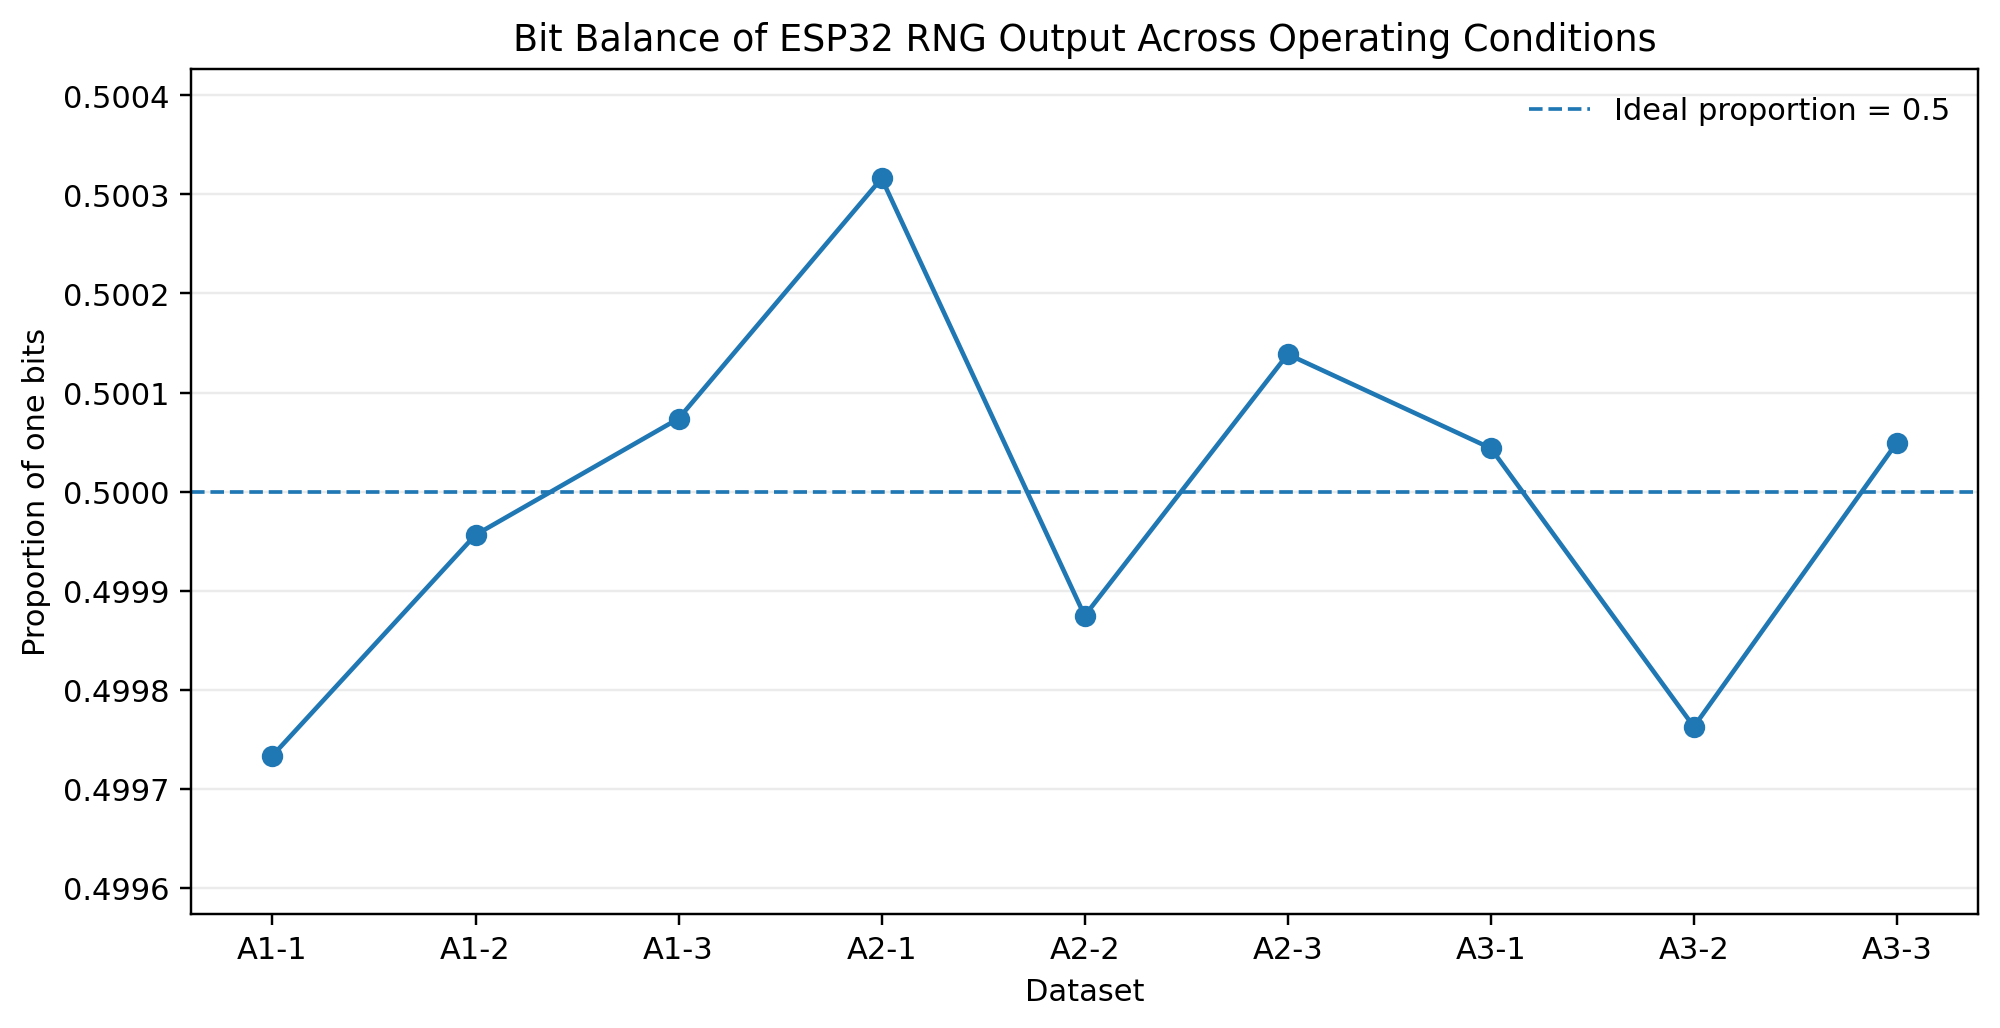
\includegraphics[width=0.85\textwidth]
        {figures/esp32_bit_proportion.png}
    \caption{Proportion of one bits in the nine 1~MiB ESP32 RNG datasets.
    The reference line at 0.5 represents the expected proportion for an
    unbiased binary sequence.}
    \label{fig:esp32_bit_proportion}
\end{figure}

\paragraph{Observations}. This did not reveal a clear statistical distinction
between the three entropy source configurations. Disabling
Wi-Fi, Bluetooth, and SAR entropy in the A1 condition did
not result in bias repeated output or reduced Shannon entropy at the RNG interface.

Similarly, enabling the SAR entropy source in A2 or the RF
subsystem in A3 did not produce an observable improvement in these basic
statistical measurements. The output from all three configurations appeared
statistically similar in the experiment.

These results alone are not sufficient to establish the amount of physical
entropy present in the ESP32 RNG. Statistical randomness in the conditioned
output does not demonstrate that fresh physical entropy is continuously being
introduced into the generator. Nevertheless, the absence of an observable
degradation in A1 provided an indication that the ESP32 might not behave
as an entropy starved device.

\subsubsection{Experiment 2: NIST SP 800-22 Statistical Evaluation}

\paragraph{Objective}

Although the initial experiment did not reveal obvious
difference between the three operating conditions, the measurements used in
Experiment 1 represent only a limited set of statistical properties.
Therefore, the NIST Statistical Test Suite (STS), was used to perform a more comprehensive statistical evaluation of the RNG output.

This was to decide whether the A1 baseline condition showed statistical deviations
that was not obvious in the first experiment and to compare these results
with the A2 and A3 conditions.

\paragraph{Dataset Preparation}

The three independently collected 1~MB datasets belonging to each operating
condition were concatenated to form one 3 MB dataset per condition. 

\begin{itemize}
    \item \textbf{A1:} baseline operation with Wi-Fi, Bluetooth, and explicit
    SAR entropy acquisition disabled;
    \item \textbf{A2:} SAR entropy source explicitly enabled; and
    \item \textbf{A3:} Wi-Fi/RF subsystem enabled.
\end{itemize}

Each combined dataset contained over 3 million bytes. The NIST STS was configured to analyse 25 independent
sequences of 1 million bits from each dataset.

The input was supplied to the test suite in binary format. All 15 statistical
test categories available in the NIST test suite were enabled.
The test parameters used were as follows,
Table~\ref{tab:nist_sts_parameters}.

\begin{table}[htbp]
    \centering
    \caption{NIST SP~800-22 test configuration}
    \label{tab:nist_sts_parameters}
    \begin{tabular}{ll}
        \toprule
        \textbf{Parameter} & \textbf{Value} \\
        \midrule
        Sequence length & 1,000,000 bits \\
        Number of sequences & 25 \\
        Input format & Binary \\
        Statistical test categories & All 15 enabled \\
        Block Frequency block length ($M$) & 128 \\
        Non-overlapping Template length ($m$) & 9 \\
        Overlapping Template length ($m$) & 9 \\
        Approximate Entropy block length ($m$) & 10 \\
        Serial block length ($m$) & 16 \\
        Linear Complexity block length ($M$) & 500 \\
        \bottomrule
    \end{tabular}
\end{table}

\paragraph{Results}

Table~\ref{tab:nist_sts_results} presents the pass proportions obtained for
the principal NIST SP~800-22 tests.

\begin{table}[htbp]
    \centering
    \caption{NIST SP~800-22 pass proportions for the three ESP32 operating
    conditions}
    \label{tab:nist_sts_results}
    \resizebox{\textwidth}{!}{
    \begin{tabular}{lccc}
        \toprule
        \textbf{Statistical Test} &
        \textbf{A1 Baseline} &
        \textbf{A2 SAR ON} &
        \textbf{A3 RF ON} \\
        \midrule

        Frequency
        & 24/25 & 25/25 & 25/25 \\

        Block Frequency
        & 25/25 & 25/25 & 24/25 \\

        Cumulative Sums
        & 24/25, 25/25
        & 25/25, 25/25
        & 25/25, 25/25 \\

        Runs
        & 25/25 & 25/25 & 25/25 \\

        Longest Run of Ones
        & 24/25 & 25/25 & 25/25 \\

        Binary Matrix Rank
        & 24/25 & 25/25 & 25/25 \\

        Discrete Fourier Transform
        & 25/25 & 25/25 & 25/25 \\

        Overlapping Template
        & 25/25 & 24/25 & 25/25 \\

        Universal Statistical
        & 25/25 & 25/25 & 25/25 \\

        Approximate Entropy
        & 24/25 & 25/25 & 23/25 \\

        Serial
        & 25/25, 25/25
        & 25/25, 25/25
        & 25/25, 24/25 \\

        Linear Complexity
        & 25/25 & 25/25 & 25/25 \\

        \bottomrule
    \end{tabular}}
\end{table}

\paragraph{Non overlapping Template and Excursion Tests}

The Non-overlapping Template test evaluated multiple templates and produuced a large collection of individual results. Most results under all 3 conditions produced pass proportions between 23/25 and 25/25.


\paragraph{Comparative Observation}.
Figure~\ref{fig:nist_sts_comparison} provides a comparison of the pass
proportions for tests across A1, A2, and A3.

\begin{figure}[htbp]
    \centering
    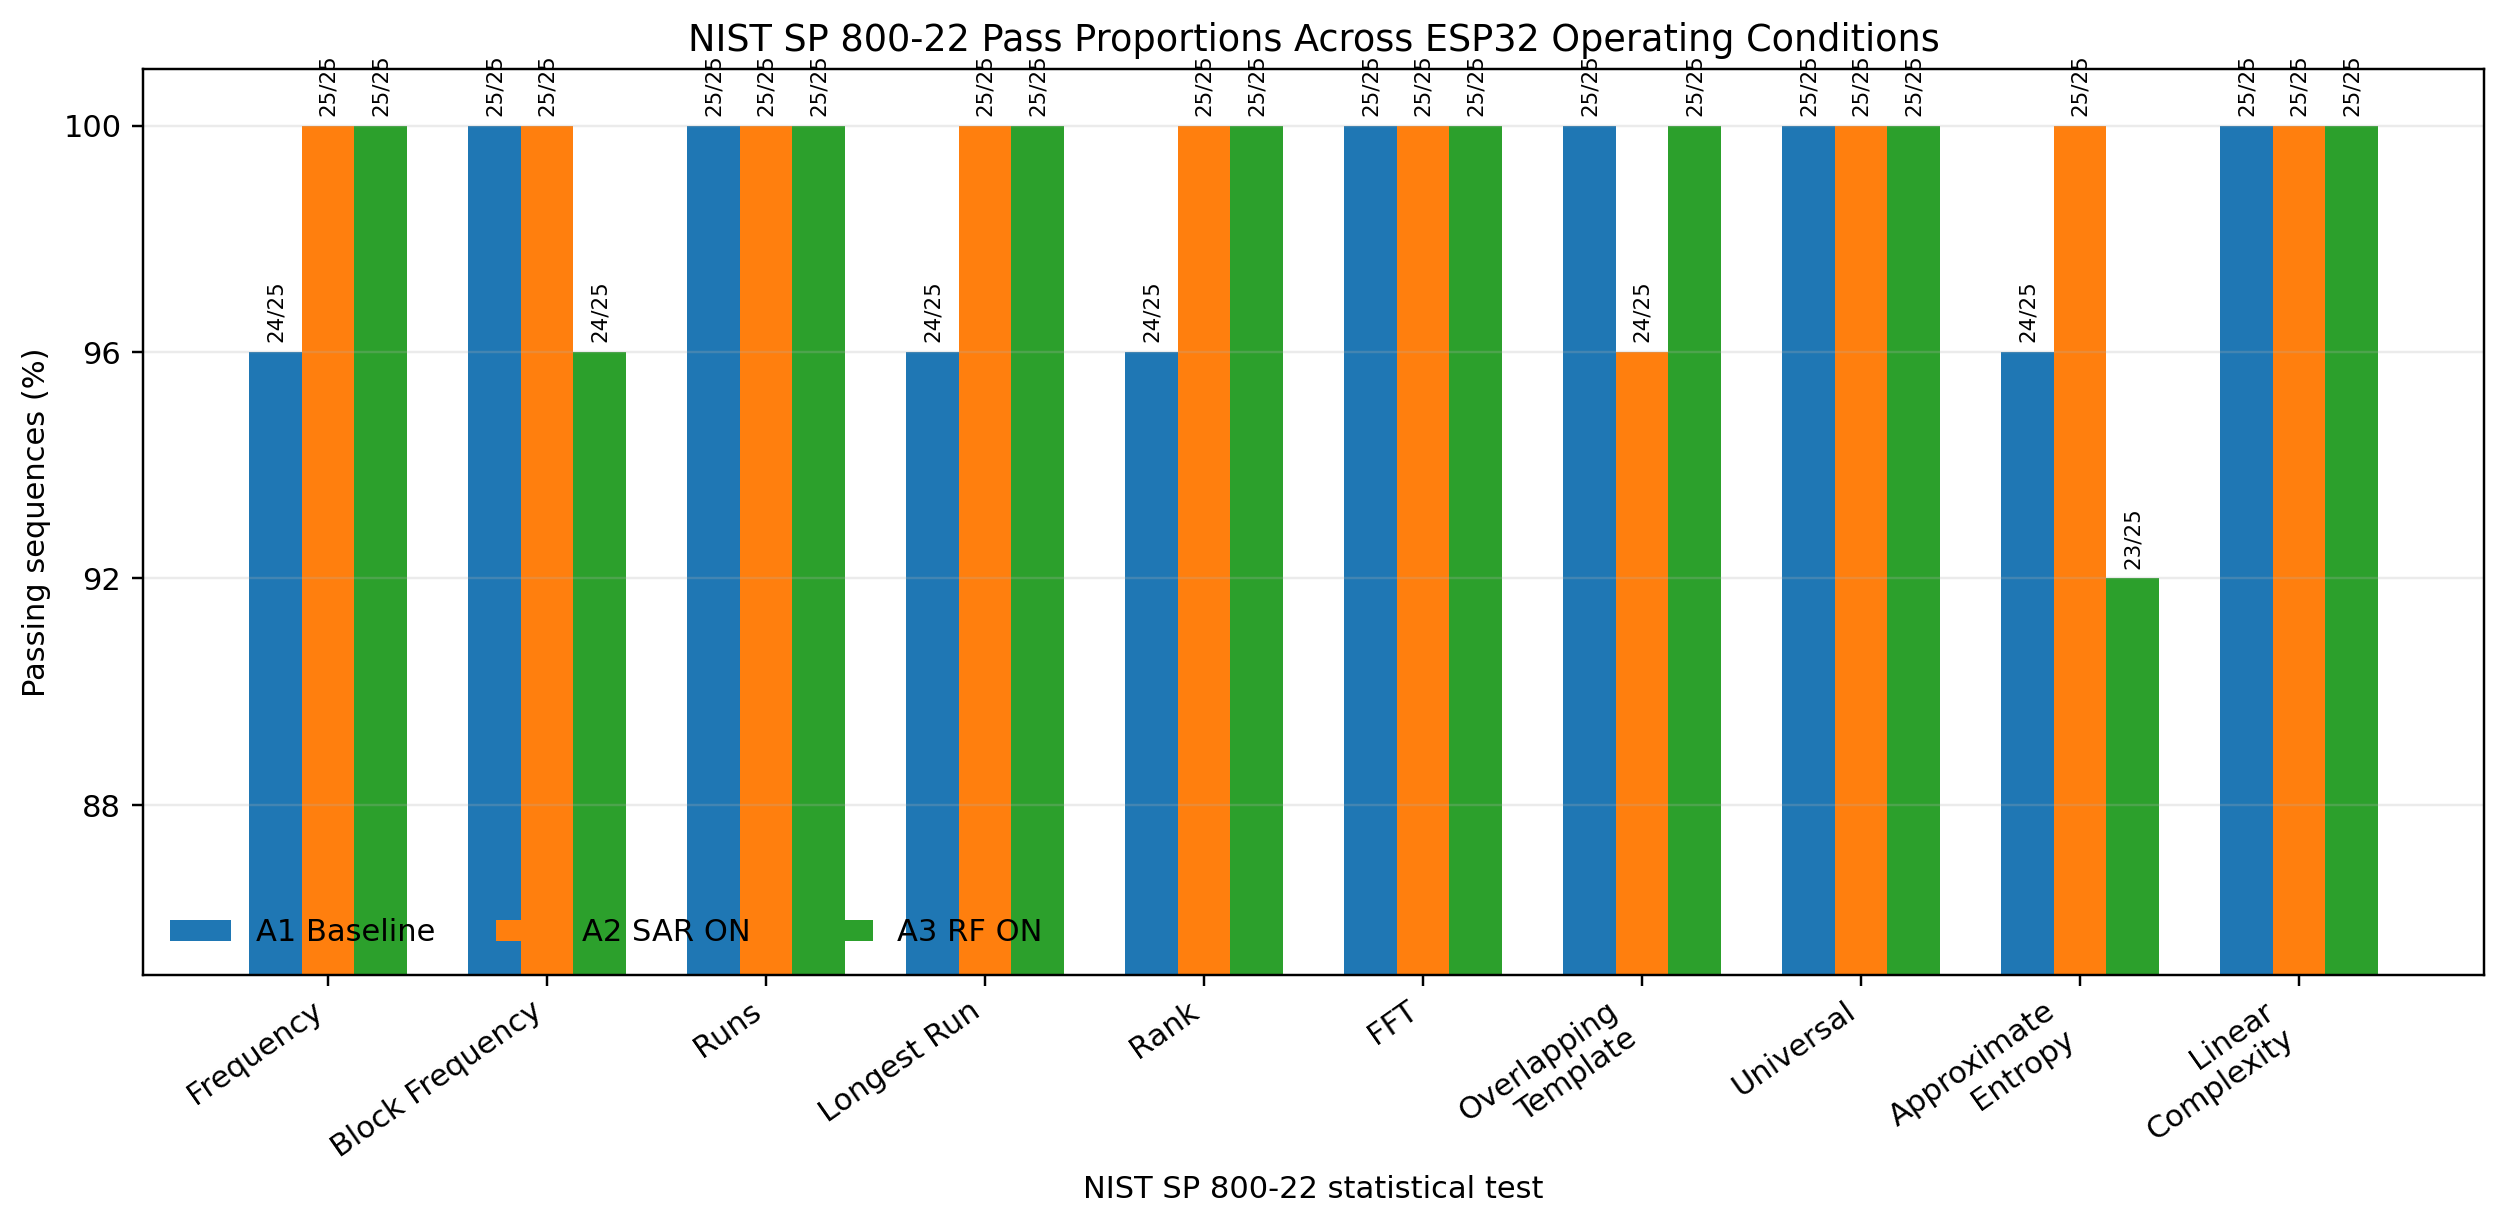
\includegraphics[width=\textwidth]
        {figures/nist_sp80022_comparison.png}
    \caption{Comparison of NIST SP~800-22 pass proportions for selected
    statistical tests across the three ESP32 operating conditions.}
    \label{fig:nist_sts_comparison}
\end{figure}

No consistent ordering was observed in which A2 or A3 outperformed the A1
baseline condition. For example, A1 produced 25/25 for Block Frequency while
A3 produced 24/25, whereas A1 produced 24/25 for Frequency while A2 and A3
produced 25/25. Similarly, A3 produced the lowest Approximate Entropy pass
proportion despite operating with the RF entropy source enabled.

Therefore, the differences observed between the three configurations did not
form a systematic pattern corresponding to the availability of a documented
continuous entropy source.

\paragraph{Observations}.The NIST SP~800-22 results did not reveal broad or systematic statistical
degradation in theESP32 RNG output under the A1 baseline
condition with the majority of test proportions comparable across A1, A2,
and A3.

However, these findings should not be interpreted as evidence that the
physical entropy available under the three conditions is equivalent. The
as NIST SP~800-22 evaluates the statistical properties of the resulting
bitstreams rather than directly measuring the physical entropy source.

These results strengthen the observation from Experiment~1.

\subsubsection{Experiment 3: NIST SP 800-90B Min-Entropy Characterization}

\paragraph{Objective}.NIST SP~800-90B entropy assessment tool was used to further atudy the unpredictability of the
ESP32 RNG output. The aim was to compare the estimated min-entropy of the board under A1, A2, and A3.

\paragraph{Method}.The same 3 MB datasets prepared for the three operating conditions were
analysed using the NIST SP~800-90B Entropy Assessment tool. Since
\texttt{esp\_fill\_random()} The conditioned
sequential data mode was used on the board. Both IID and non-IID assessments were performed using 8 bit input symbols.

\begin{table}[htbp]
    \centering
    \caption{NIST SP~800-90B min-entropy estimates for ESP32 RNG output}
    \label{tab:sp80090b_results}
    \begin{tabular}{lcc}
        \toprule
        \textbf{Condition} &
        \textbf{IID $h'$} &
        \textbf{Non-IID $h'$} \\
        \midrule
        A1 -- Baseline & 0.999032 & 0.929709 \\
        A2 -- SAR ON   & 0.998943 & 0.920188 \\
        A3 -- RF ON    & 0.999121 & 0.929736 \\
        \bottomrule
    \end{tabular}
\end{table}

\begin{figure}[htbp]
    \centering
    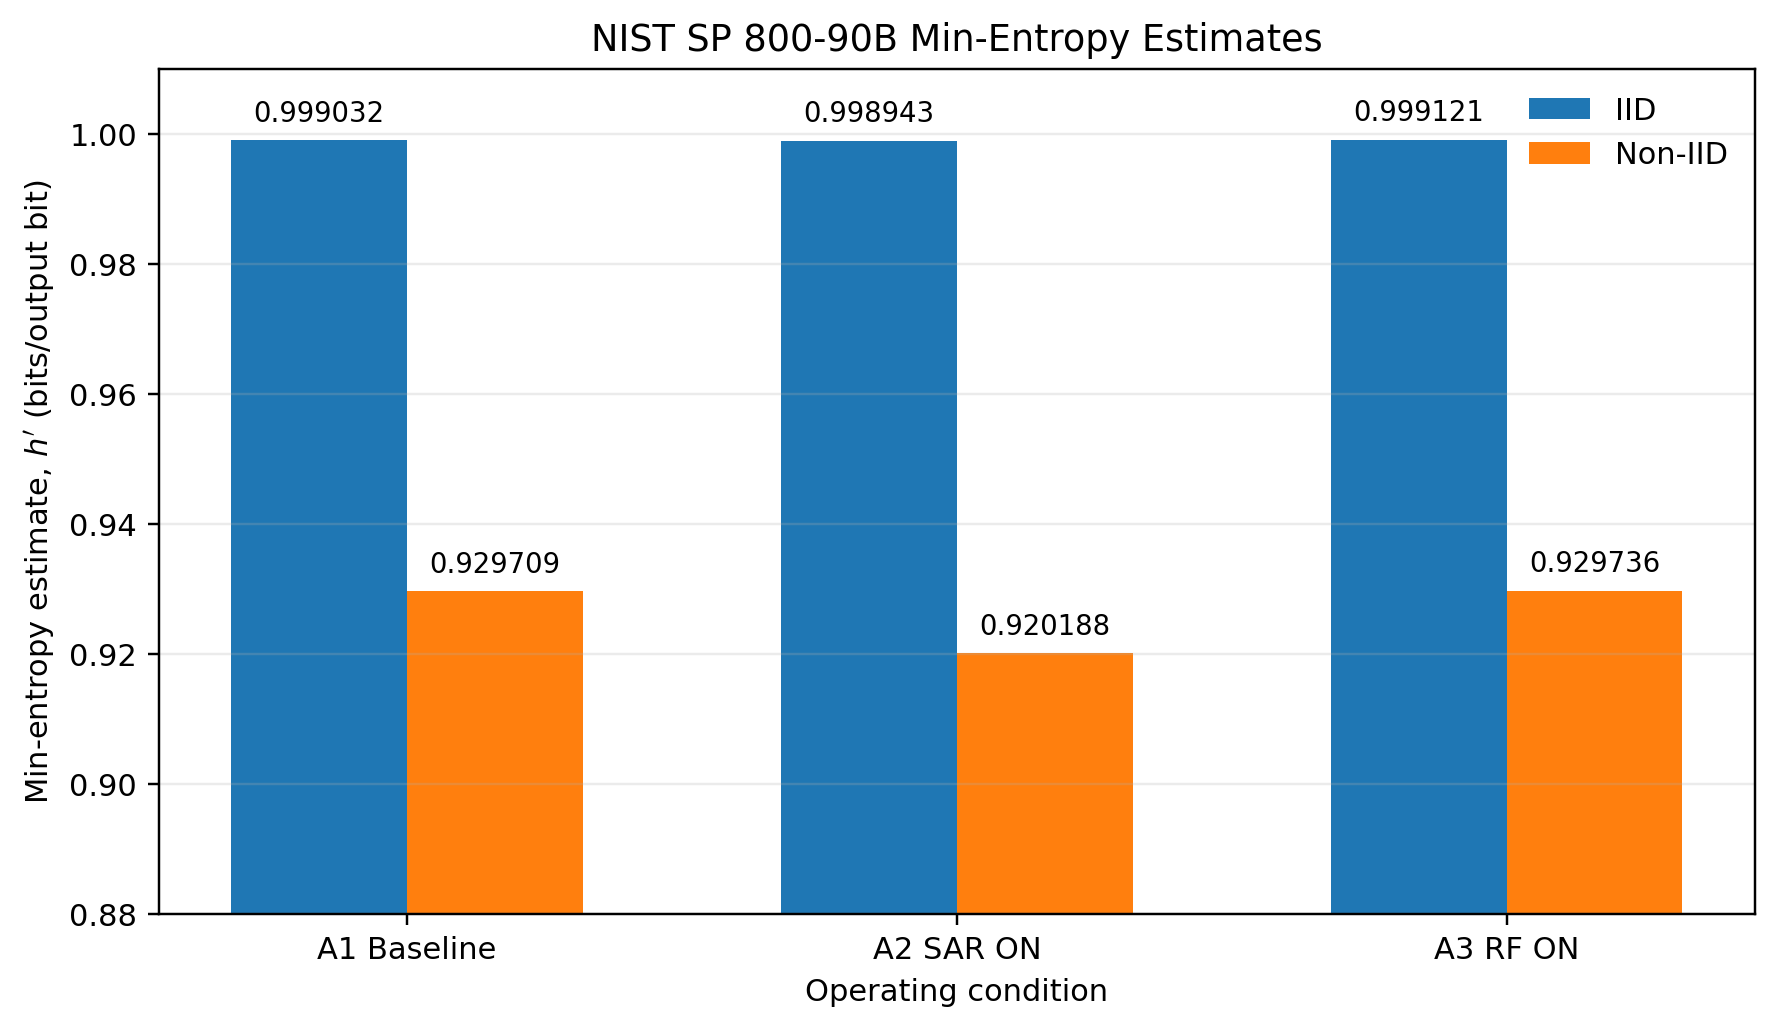
\includegraphics[width=0.75\textwidth]
        {figures/nist_sp80090b_comparison.png}
    \caption{Comparison of NIST SP~800-90B IID and non-IID min-entropy
    estimates for the three ESP32 operating conditions.}
    \label{fig:sp80090b_comparison}
\end{figure}

\paragraph{Observations}. All three datasets passed the IID assessment. The IID estimates were close to
1 bit per output bit, ranging from 0.998943 to 0.999121. The conservative
non-IID assessment produced estimates of 0.929709, 0.920188, and 0.929736 for
A1, A2, and A3 respectively.

This analysis provides further evidence that no obvious weakness was
detected in the conditioned RNG output of the A1 baseline configuration. The analysis was performed on the conditioned output returned by \texttt{esp\_fill\_random()} rather than the noise samples.

Therefore, the results only characterize the output visible to the
application. Thus enabling the SAR or RF entropy source did
not produce a clear improvement over the A1 baseline output.

\subsubsection{Experiment 4: Sustained RNG Stress Test}

\paragraph{Objective}. The previous experiments analysed fixed RNG datasets. This experiment was
conducted to determine whether continuously requesting random data for an
extended period would cause reduction in RNG performance or output quality.

\paragraph{Method}.The ESP32 RNG was continuously stressed for approximately 10 minutes under
each of the A1, A2, and A3 operating conditions. Random data was generated
using repeated 64 byte calls to \texttt{esp\_fill\_random()}.

Measurements were recorded over 60 consecutive 10-second windows with the
experiment monitored the amount of data generated, number of RNG calls,
generation time, throughput, call latency, proportion of one bits, and
frequency of zero valued bytes. The Random data was analysed locally on the ESP32
rather than transmitted over the serial connection, avoiding UART transfer
speed from affecting the results.

\begin{table}[htbp]
    \centering
    \caption{Results of the 10-minute sustained RNG stress test}
    \label{tab:rng_stress_results}
    \resizebox{\textwidth}{!}{
    \begin{tabular}{lccc}
        \toprule
        \textbf{Metric} &
        \textbf{A1 Baseline} &
        \textbf{A2 SAR ON} &
        \textbf{A3 RF ON} \\
        \midrule
        Generated data (bytes)
        & 87,424,384 & 87,425,984 & 87,429,120 \\

        RNG calls
        & 1,366,006 & 1,366,031 & 1,366,080 \\

        RNG generation time (s)
        & 529.987 & 529.843 & 529.598 \\

        Throughput (B/s)
        & 164,955.60 & 165,003.56 & 165,085.79 \\

        Calls $\geq$ 1 ms
        & 0 & 0 & 0 \\
        \bottomrule
    \end{tabular}}
\end{table}

\paragraph{Observations}
Approximately 83~MB of random data was generated under each condition,
resulting in approximately 250~MB across the complete experiment. More than
1.36 million RNG calls were made in each individual test. The average throughput remained close to 165~kB/s for all three conditions.
No RNG call exceeded 1~ms, and no progressive reduction in throughput was
observed during the 10-minute test period with the measured bit proportions and
zero-byte frequencies also remained stable throughout the experiment.

This does not prove that physical entropy was being generated at the same rate
under all three conditions. However, from the application perspective, heavy
and continuous RNG usage did not produce an observable degradation in the
ESP32 RNG output or performance.


\subsubsection{Experiment 5: Cryptographic Key Generation Stress Testing}

\paragraph{Objective}
This experiment evaluated the RNG under a more realistic cryptographic
workload by repeatedly generating P 256 elliptic-curve key pairs.

\paragraph{Method}
P 256 key pairs were repeatedly generated using the mbedTLS cryptographic
library under the A1, A2, and A3 operating conditions. Each condition was tested for approximately 10 minutes. The number of
successful and failed key generations and the average key-generation time were
also recorded.

\begin{table}[htbp]
    \centering
    \caption{P-256 key-generation stress-test results}
    \label{tab:p256_results}
    \resizebox{\textwidth}{!}{
    \begin{tabular}{lccc}
        \toprule
        \textbf{Metric} &
        \textbf{A1 Baseline} &
        \textbf{A2 SAR ON} &
        \textbf{A3 RF ON} \\
        \midrule
        Successful keys & 2401 & 2401 & 1740 \\
        Failed keys & 0 & 0 & 0 \\
        RNG calls & 4802 & 4802 & 3480 \\
        RNG output (bytes) & 153,664 & 153,664 & 111,360 \\
        RNG output per key & 64 & 64 & 64 \\
        Average key-generation time (ms)
            & 246.109 & 246.227 & 347.417 \\
        Average RNG time per key ($\mu$s)
            & 391.23 & 391.29 & 399.14 \\
        \bottomrule
    \end{tabular}}
\end{table}

\paragraph{Observations}
A total of 6,542 P-256 key pairs were successfully generated across the three
conditions, with no key-generation failures. Each key generation required two
RNG calls and 64 bytes of RNG output.

A1 and A2 showed almost identical key-generation times of approximately
246~ms. Key generation was slower in A3, averaging approximately 347~ms.
However, the RNG itself required only approximately 399~$\mu$s per key in A3,
compared with approximately 391~$\mu$s in A1 and A2. Therefore, additional execution time in A3 occurred outside the RNG operation. Therefore, the experiment did not provide evidence of RNG exhaustion under a
repeated cryptographic workload.

\subsubsection{Implications of the ESP32 Evaluation}

The ESP32 experiments were conducted to determine whether the device could
serve as an entropy constrained platform for the purpose of my research. Table~\ref{tab:esp32_overall_findings} summarizes
the main findings.

\begin{table}[htbp]
    \centering
    \caption{Summary of ESP32 experimental findings}
    \label{tab:esp32_overall_findings}
    \resizebox{\textwidth}{!}{
    \begin{tabular}{lll}
        \toprule
        \textbf{Experiment} & \textbf{Main Observation} &
        \textbf{Outcome} \\
        \midrule

        Initial RNG characterization &
        A1, A2 and A3 produced similar statistical properties &
        No clear A1 degradation \\

        NIST SP~800-22 &
        No broad or systematic difference between conditions &
        No clear A1 weakness detected \\

        NIST SP~800-90B &
        Similar conditioned-output estimates across conditions &
        No clear A1 weakness detected \\

        Sustained RNG stress &
        Approx. 250~MiB generated with stable performance &
        No observable exhaustion \\

        P-256 key generation &
        6,542 successful keys with no failures &
        No observable RNG failure \\

        Boot/reset testing &
        No repeated samples or clear startup degradation &
        No application-visible boot-time weakness \\

        \bottomrule
    \end{tabular}}
\end{table}

The findings do not prove that the same amount of physical entropy is
available under all three conditions. The experiments mainly observed the
conditioned output provided by the ESP32 RNG interface, while the internal
physical entropy source and RNG state are not directly accessible. Therefore,
differences in physical entropy availability may not be visible through these
output level tests.

Therefore the experiments show that the ESP32 does not exhibit an obvious
application visible entropy limitation under the tested conditions. As a
result, it is not considered a suitable primary example of an entropy-starved
device for evaluating my proposed collaborative entropy sharing mechanism.


Therefore, the next stage my platform evaluation focused on a more
constrained microcontroller without a dedicated hardware RNG. This
motivated the evaluation of the STM32F103 as the next candidate platform.

\subsection{Evaluation of the STM32F103 (``Blue Pill'') Platform}
 
\subsubsection{Motivation for Changing the Target Platform}
 
My initial plan was to build and evaluate the proposed entropy sharing mechanism on ESP32 boards. Evaluating the ESP32 showed that it already provides a hardware random number generator and analog entropy sources, draws considerably more power than a typical constrained node (see \citet{espressif2026rng}). On such a platform the problem that this research addresses which is that a device that cannot obtain sufficient entropy locally does not really occur, so the ESP32 would not be a convincing testbed for collaborative entropy sharing.

 
Following discussions, the target platform was changed to a low power microcontroller with no dedicated hardware random number generator that can still run a real time operating system and used in the IoT industry. The STM32F103C8T6 (the ``Blue Pill'') was selected because the STM32F103 family does not include a hardware RNG peripheral \citep{st2021rm0008}, it is inexpensive and available locally, it has 20~KB of RAM and 64~KB of flash which would be enough for a hash function, a lightweight protocol and an RTOS such as FreeRTOS yet small enough to be genuinely resource constrained. The platform can also be extended with a low cost radio module for peer to peer communication. Boards with a built in hardware RNG (for example the Raspberry Pi Pico 2 and other STM32 families) were rejected for the same reason as the ESP32.
 
\subsubsection{Aim of the Experiments}
 
The experiments which I conducted are shown in in this subsection and they establish, with measurements how weak a single device's randomness is on this platform. They address four questions,
 
\begin{enumerate}
    \item Are the random values produced after boot predictable when a developer seeds a software generator in ways that are common in practice?
    \item Can statistical analysis of the generator's output reveal this weakness?
    \item How much min-entropy do the local entropy sources of the chip provide, and how stable is it?
    \item How does the one time source available on the chip (SRAM start-up state) compare with the other sources?
\end{enumerate}
 
The results provide the baseline against which the proposed collaborative mechanism will later be evaluated (see the Evaluation Plan) and motivate several design decisions.
 
\subsubsection{Experimental Setup}
 
\paragraph{Hardware and tools.} Two Blue Pill boards (B1 and B2) were used. Boards were programmed through an ST-Link V2 programmer and connected to a laptop through a CH340 USB--UART adapter on USART2 (115200~baud). Firmware was written in C++ using PlatformIO with the Arduino STM32 core. Captured data were processed with Python scripts. Min-entropy was estimated with the non-IID track of the open source NIST SP~800-90B Entropy Assessment tool \citep{turan2018sp80090b} run under Ubuntu on WSL.
 
\paragraph{Board identity.} The identity of the two chips was read from the debug and device-ID registers (Table~\ref{tab:bp_ids}). Both boards are marked STM32F103C8T6, report 64~KB of flash and have different unique IDs, whose final word is identical, which suggests the boards come from the same production batch. The firmware reads a core identifier of \texttt{0x412FC231} and STM32CubeProgrammer reported the device ID as \texttt{0x410} over the debug port.
 
\begin{table}[htbp]
\centering
\small
\caption{Identity of the two boards used}

\label{tab:bp_ids}
\begin{tabularx}{\textwidth}{@{}p{0.27\textwidth}XX@{}}
\toprule
 & \textbf{Board 1 (B1)} & \textbf{Board 2 (B2)} \\
\midrule
Chip marking & STM32F103C8T6 & STM32F103C8T6 \\
Flash size (read by firmware) & 64 KB & 64 KB \\
Debug ID (firmware read) & 0x307 & 0x307 \\
Core ID (CPUID) & 0x412FC231 & 0x412FC231 \\
Device ID (CubeProgrammer) & 0x410 & 0x410 \\
Unique ID & 00670039-50000014-4E54574D & 00740029-5000000D-4E54574D \\
\bottomrule
\end{tabularx}
\end{table}
 
\paragraph{Data capture and integrity checks.} Raw 12 bit ADC readings were streamed to the laptop and stored as binary files of one million samples per run. After early captures were found to be vulnerable to a one byte misalignment, a self synchronising framing was introduced (each reading is sent as two bytes carrying marker bits) and the capture script rejects any file in which the framing breaks. Further checks were applied to every file including range checks, scan for repeated 16 byte windows, counting of start markers in stream captures, and SHA-256 hashes of the saved files. Captures that failed a check, or that were later found to have been made in an invalid configuration were excluded from all results. Every capture were also relevantly logged for reference.
 
\paragraph{Entropy estimation.} The NIST tool accepts at most 8 bits per sample, so 12 bit readings were reduced to 8 bits. For the floating and grounded ADC pin the values were clipped at 255 (fewer than 1\% of samples reached 256 in every run except one, for which a wrapped version was also analysed and the lower result reported). For the internal temperature sensor whose readings span only about a dozen values around 1720, the minimum value of each file was subtracted so that no information was lost. Every reported value is the tool's final figure, $\min(H_{\mathrm{original}}, 8\,H_{\mathrm{bitstring}})$ (the lowest of its estimators), expressed in bits per 8 bit sample. A perfect source would score 8.
 
\subsubsection{Experiment 1: Predictability of Boot-Time Seeding}
 
\paragraph{Method.} A software pseudo random generator needs a seed, and on a device without a hardware RNG developers commonly seed it with a constant, the system time, or a single analog reading. For each of five seeding modes the firmware seeded the standard \texttt{random()} function, printed the first 64 bits it produced, and rebooted itself. 100 boots were captured per mode on each board. The modes were: (0) no seed, (1) a fixed seed (12345), (2) \texttt{millis()}, (3) \texttt{micros()}, and (4) one \texttt{analogRead} of a floating pin. Resets were software resets and not power cycles.
 
 
\begin{table}[htbp]
\centering
\small
\caption{Distinct 64-bit outputs over 100 boots per setting}
\label{tab:bp_e1}
\begin{tabularx}{\textwidth}{@{}llXXX@{}}
\toprule
\textbf{Mode} & \textbf{Seed} & \textbf{B1 distinct} & \textbf{B2 distinct} & \textbf{Same output on both boards?} \\
\midrule
0 & none & 1 & 1 & Yes \\
1 & fixed (12345) & 1 & 1 & Yes \\
2 & \texttt{millis()} & 1 & 1 & Yes \\
3 & \texttt{micros()} & 1 & 1 & Yes \\
4 & one \texttt{analogRead} & 19 (most common 17\%) & 6 (most common 42\%) & No (no value in common) \\
\bottomrule
\end{tabularx}
\end{table}
 
\paragraph{Observations.} In modes 0 to 3, all 400 boots produced the same value on both boards, so every device running this firmware would generate the same ``random'' numbers after boot. Mode 2 gave exactly the same output as mode 0, which suggests that \texttt{millis()} is still zero when the seed is taken. Seeding with one analog reading produced some variety but only 19 and 6 distinct outputs, and the most common output occurred in 17\% and 42\% of boots. Using the most common value's share, the effective entropy of this seed is roughly 2.6~bits on B1 and 1.3~bits on B2. The two boards produced entirely different sets of outputs, so the floating pin behaves differently from board to board.
 
\subsubsection{Experiment 2: A Predictable Stream Passes Entropy Estimation}
 
\paragraph{Method.} To test whether output statistics can reveal the weakness above, the generator was seeded with a fixed value (12345) and 1,000,000 bytes of its output were captured from each board and assessed with the NIST tool. Capture integrity was checked by scanning for repeated windows (none found).
 
\paragraph{Results.} The two captured files were byte for byte identical (identical SHA-256 hashes), although they came from two physically different boards. The NIST tool estimated a min-entropy of 6.97 bits per byte for the stream ($H_{\mathrm{original}}=7.85$, $H_{\mathrm{bitstring}}=0.871$ per bit), about 87\% of the maximum, although its true entropy is zero because it is fully determined by the firmware.
 
\paragraph{Discussion.} This tool is designed for physical noise sources and not for the output of a pseudo random generator, so this is not a fault of the tool. It does show that analysing the output of a generator cannot reveal a lack of unpredictability, which is why entropy has to be assessed at the source, a point also made for the ESP32 by \citep{blancoromero2026bootstrap}. A first capture of this stream, which contained a repeated segment (most likely because the board restarted during the capture), produced an estimate of only 0.0012 bits per byte, showing how strongly the repetition sensitive estimators react to repeated data. The capture was discarded and the stream was recaptured and verified.
 
\subsubsection{Experiment 3: Key Recovery from Weak Seeding}
 
\paragraph{Method.} A 128-bit value (eight 16-bit outputs of \texttt{random()}) was generated at each boot using mode 4 of Experiment~1 (one \texttt{analogRead} as the seed), and 500 boots were captured on B1. An attacker who knows the firmware was then simulated. The same code was run for every possible seed from 1 to 4095 (a 12-bit reading), and the resulting 4,095 candidate values were stored in a lookup table (generated in about 15 seconds). The board itself was used to generate the table, avoiding assumptions about the internals of the generator.
 
\paragraph{Results.} Only five distinct 128-bit values occurred in the 500 boots, and all 500 were found in the table. The seeds actually used were five adjacent readings (2099 to 2103), with counts of 74, 99, 136, 104 and 87 respectively; the most common seed occurred in 27\% of boots, which corresponds to about 1.9 bits of effective entropy for a nominally 128-bit value.
 
\paragraph{Discussion.} This demonstrates the failure mode reported for deployed devices by \citet{heninger2012mining} and \citet{mowery2013entropics}, without needing a full cryptographic key generation on the device. The recovery is instant, and it assumes only that the attacker knows the firmware and the way the seed is formed.
 
\subsubsection{Experiment 4: Min-Entropy of the Raw Local Sources}
\label{sec:bp_raw}

\paragraph{Method.} Three analogue sources were sampled with the 12-bit ADC: (a) a floating pin (PA0, unconnected), (b) the same pin firmly tied to ground as a control, and (c) the chip's internal temperature sensor. For each source, three runs of one million samples were captured on each board and assessed. Floating-pin runs on B1 fall into two groups: r1--r3, captured with the original framing and validated by range checks, and another set r4--r6, captured later with the final framing after the board had been re-seated on the breadboard. These groups were in different operating regimes (mean reading about 43 and 57 respectively), so they are reported separately.
  
\begin{table}[htbp]
\centering
\small
\caption{Min-entropy per 8-bit sample for each source (1,000,000 samples per run)}
\label{tab:bp_e2}
\begin{tabularx}{\textwidth}{@{}llXXX@{}}
\toprule
\textbf{Source} & \textbf{Board / runs} & \textbf{Run 1} & \textbf{Run 2} & \textbf{Run 3} \\
\midrule
Floating pin & B1, r1--r3 (original framing) & 1.865 & 2.359 & 2.385 \\
Floating pin & B1, r4--r6 (final framing) & 1.604 & 1.602 & 1.604 \\
Floating pin & B2 & 1.139 & 1.191 & 1.095 \\
Temperature sensor & B1 & 1.297 & 1.246 & 1.229 \\
Temperature sensor & B2 & 1.040 & 1.114 & 0.966 \\
Grounded pin (control) & B1 & 0.0095 & 0.0078 & 0.0101 \\
Grounded pin (control) & B2 & 0.00015 & 0.00009 & 0.00016 \\
\bottomrule
\end{tabularx}
\end{table}
 
\begin{figure}[htbp]
\centering
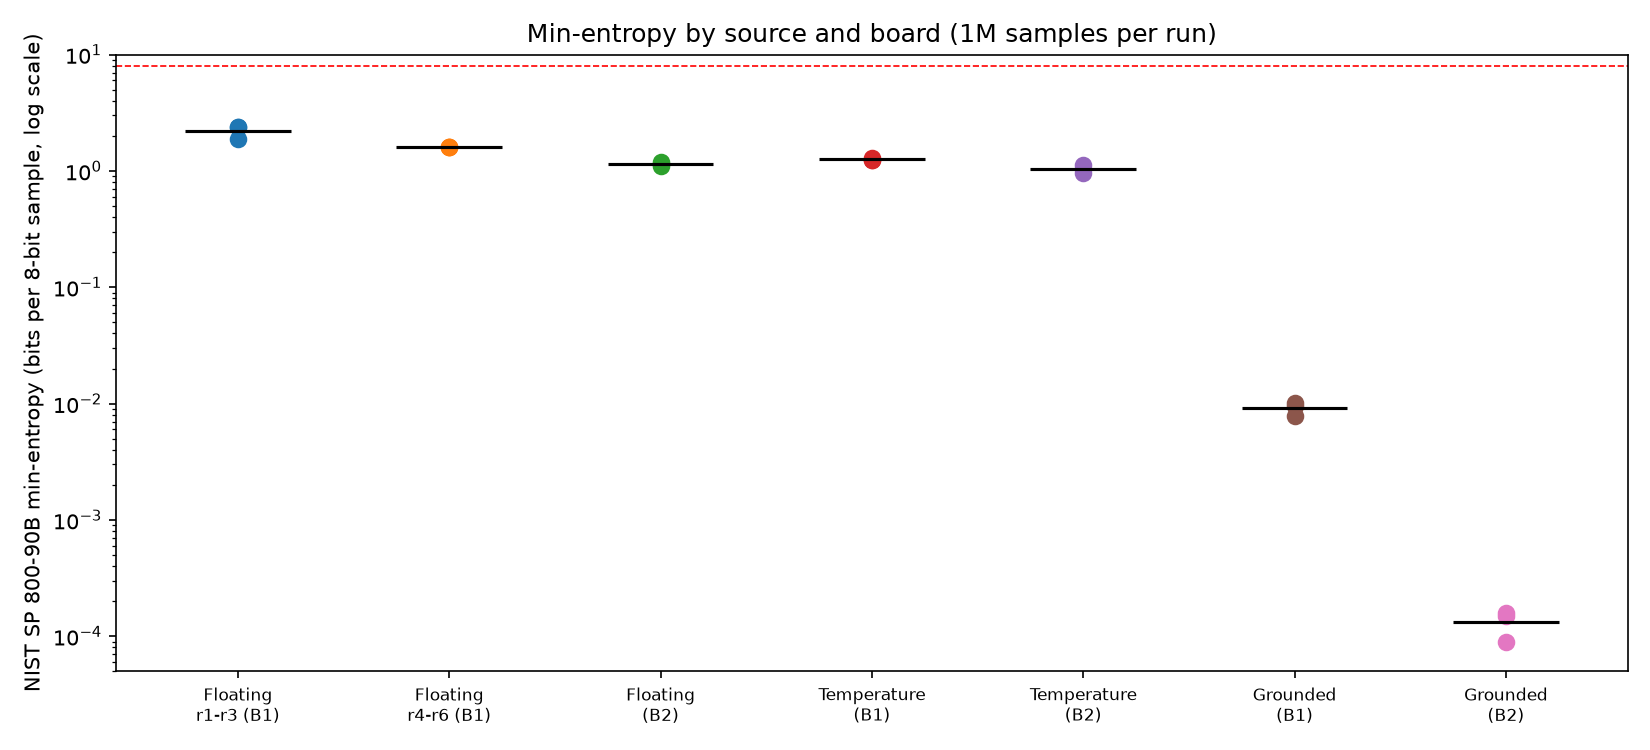
\includegraphics[width=\textwidth]{figures/summary_both_boards.png}
\caption{Min-entropy (NIST SP~800-90B, bits per 8-bit sample, logarithmic scale) for every valid run on both boards. Dashed line marks the ideal value of 8 bits.}
\label{fig:bp_summary}
\end{figure}
 
\paragraph{Observations.}
\begin{itemize}
    \item \textbf{All local analogue sources are weak.} The floating pin and the temperature sensor give roughly 1 to 2.4 bits of min-entropy per 8-bit sample, between 12\% and 30\% of the ideal value of 8.
    \item \textbf{The ADC contributes almost nothing on its own.} With the pin grounded the entropy falls to between 0.0001 and 0.01 bits, so whatever the floating pin provides comes from the signal on the pin and not from the converter. This does not show that the signal is unpredictable because it may be partly produced by the board itself (Experiment~6).
    \item \textbf{Consecutive samples are dependent.} In the runs examined, the limiting estimators were sequence based (the MultiMMC predictor or the longest repeated substring estimate for the floating pin, and the compression estimate for the temperature sensor) not the simple most common value estimate. Estimating entropy from value frequencies alone would be an overstatement. The histogram and bit bias plots in Figures~\ref{fig:bp_float_b1}, \ref{fig:bp_float_b2} and \ref{fig:bp_temp} show how concentrated the readings are with only the lowest few bits of each reading varying.
    \item \textbf{Results vary between boards and setups.} Board 2 measured lower than Board 1 for both the floating pin and the temperature sensor, and the floating pin on B1 measured between 1.60 and 2.39 bits depending on the setup. Since the two boards are probably from the same batch and were set up at different times, this should be read as an observation and not as a property of the chip.
\end{itemize}
 
\begin{figure}[htbp]
\centering
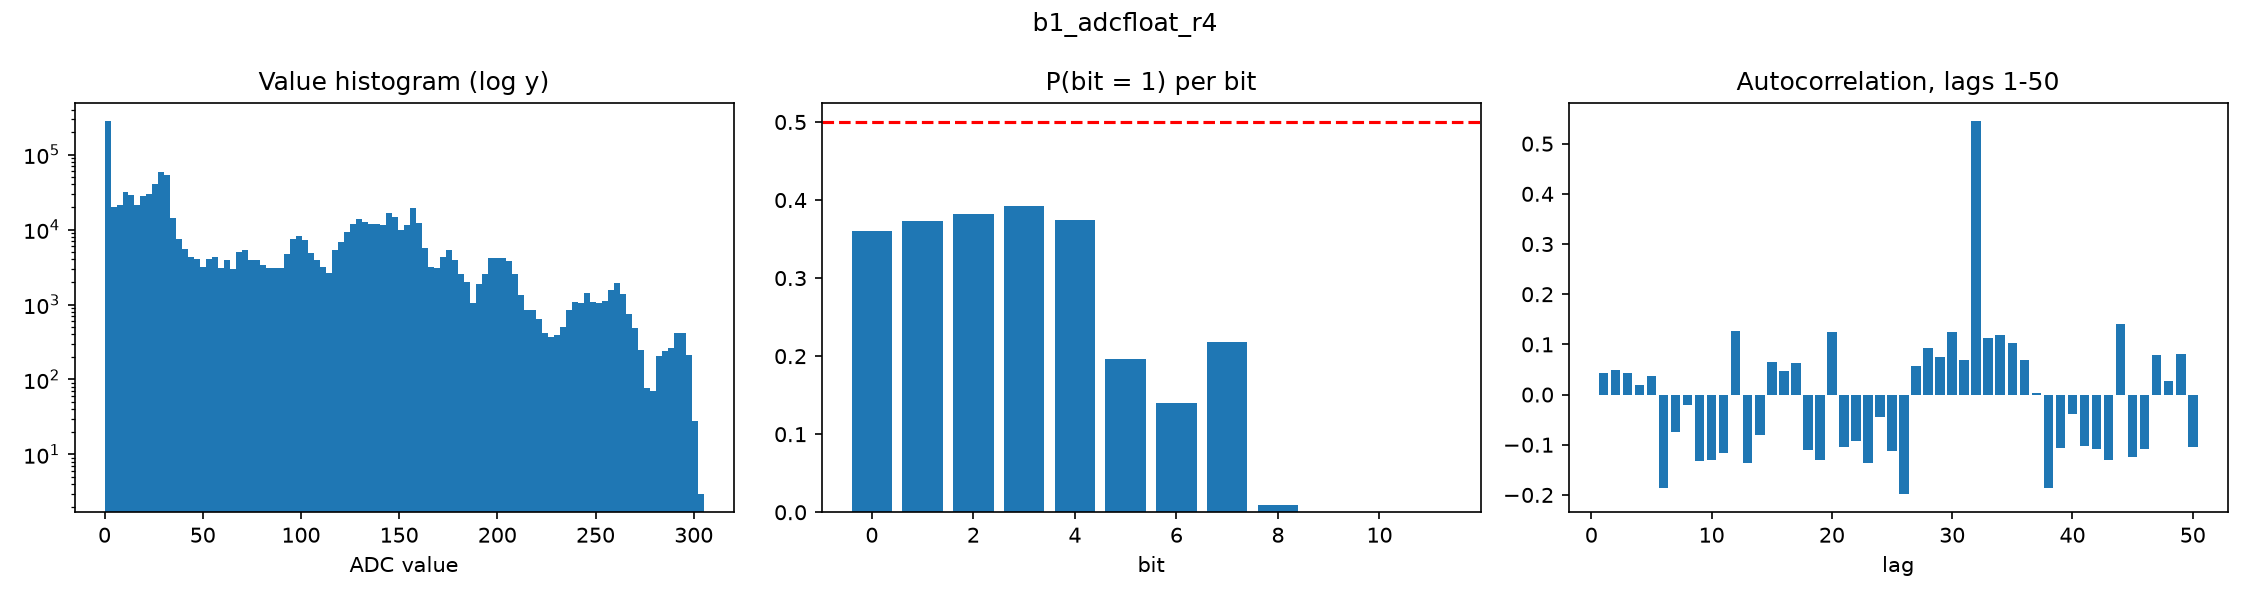
\includegraphics[width=\textwidth]{figures/b1_adcfloat_r4.png}
\caption{Board 1, floating pin (run r4): value histogram (log scale), probability of each bit being 1, and autocorrelation for lags 1 to 50.}
\label{fig:bp_float_b1}
\end{figure}
 
\begin{figure}[htbp]
\centering
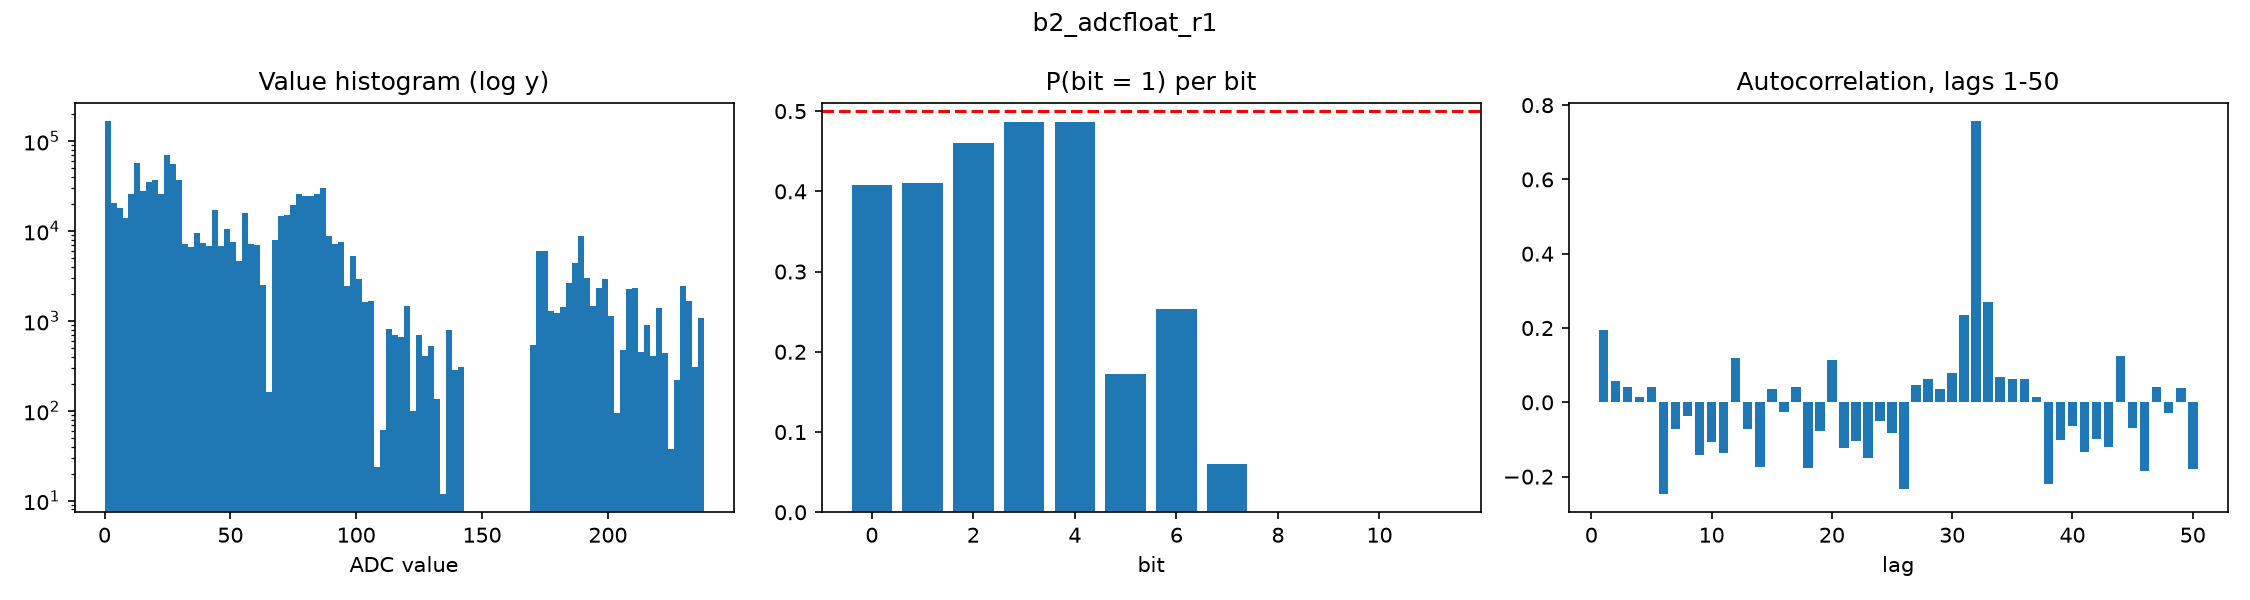
\includegraphics[width=\textwidth]{figures/b2_adcfloat_r1.png}
\caption{Board 2, floating pin (run 1), same panels as Figure~\ref{fig:bp_float_b1}.}
\label{fig:bp_float_b2}
\end{figure}
 
\begin{figure}[htbp]
\centering
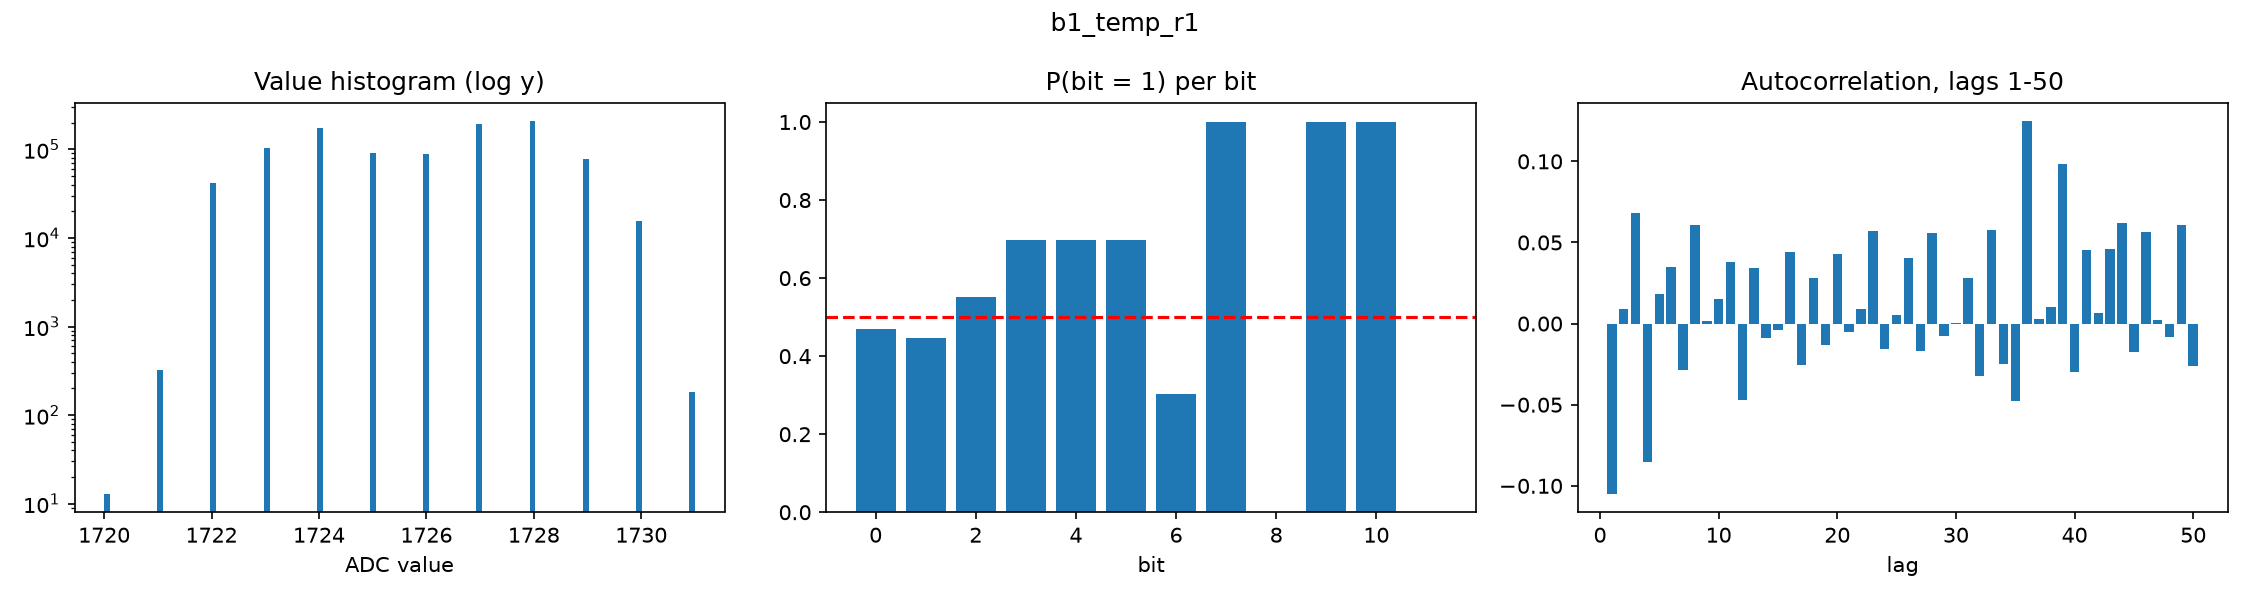
\includegraphics[width=\textwidth]{figures/b1_temp_r1.png}
\caption{Board 1, internal temperature sensor (run 1). The readings span only 12 distinct values.}
\label{fig:bp_temp}
\end{figure}
 
\begin{figure}[htbp]
\centering
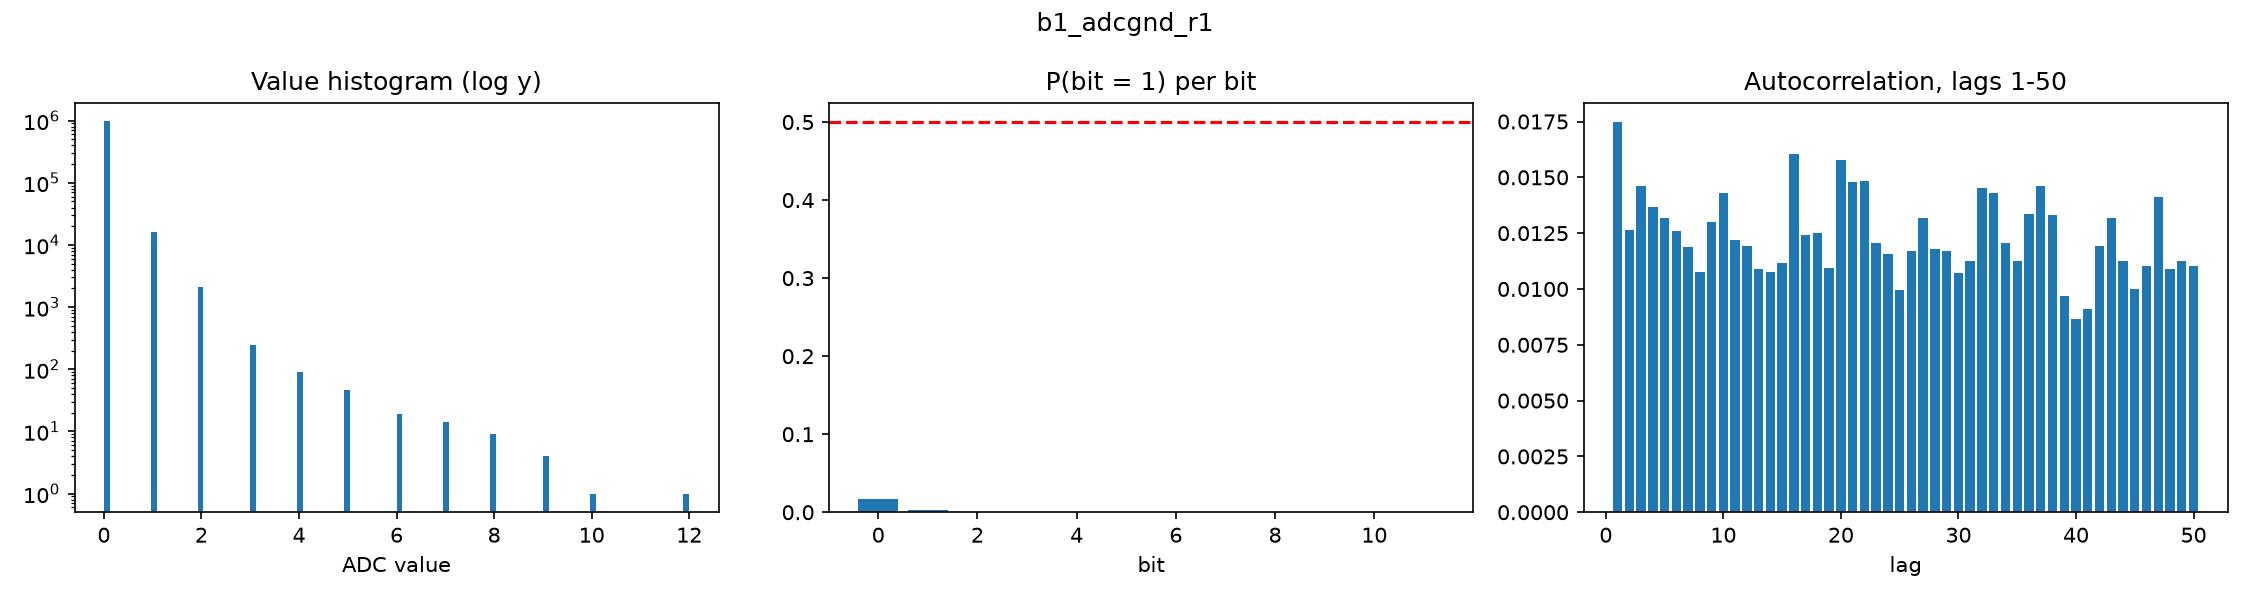
\includegraphics[width=\textwidth]{figures/b1_adcgnd_r1.png}
\caption{Board 1, grounded pin (run 1). Almost all readings are zero, and the autocorrelation values are very small.}
\label{fig:bp_gnd}
\end{figure}
 
\subsubsection{Experiment 5: Sensitivity of the Floating Pin to its Surroundings}
\label{sec:bp_context}
 
\paragraph{Method.} Literature on sensor based entropy warns that such sources can be influenced by an adversary \citep{hennebert2021entropy}. To test this on the floating pin of B1, one million samples were captured under five conditions with the board and wiring left untouched between captures: nothing nearby (before), a hand about 2~cm from the pin, a phone with its hotspot active about 5~cm away, a 10~cm loose wire attached to the pin as an antenna, and nothing nearby again (after). Two repeats of this experiment had been run with one before the board was removed and re-seated, and are reported for comparison.
 
\paragraph{Results.} Table~\ref{tab:bp_e3} gives the results.
 
\begin{table}[htbp]
\centering
\small
\caption{Min-entropy of the floating pin of B1 under different conditions}
\label{tab:bp_e3}
\begin{tabularx}{\textwidth}{@{}Xcc@{}}
\toprule
\textbf{Condition} & \textbf{Setup A (before re-seating)} & \textbf{Setup B (after re-seating)} \\
\midrule
Nothing nearby (before) & 1.602 & 1.281 \\
Hand about 2 cm away & 1.760 & 1.291 \\
Phone hotspot about 5 cm away & 1.655 & 1.289 \\
Nothing nearby (after) & --- & 1.292 \\
10 cm wire on the pin & --- & 1.208 (clipped), 1.199 (wrapped) \\
\bottomrule
\end{tabularx}
\end{table}
 
\paragraph{Observations.}
\begin{itemize}
    \item In Setup B, the two ``nothing nearby'' captures agree within 0.011 bits, so the source did not drift during the session. A hand and a phone produced values (1.291, 1.289) within the same 0.011 bits, so \textbf{no effect of a nearby hand or phone could be detected.}
    \item The \textbf{antenna wire} lowered the min-entropy by about 0.09 bits and shifted the mean reading from about 66 to 79 (with 10\% of samples above 255), as shown in Figure~\ref{fig:bp_wire}. Adding a pickup antenna did not noticeably increase the entropy. This was observed in a single capture.
    \item \textbf{Re-seating the board changed the result more than the stimuli.} The same ``nothing nearby'' condition measured 1.60 bits before and 1.29 bits after, with the mean reading moving from about 57 to 66. Comparisons are therefore only valid within a setup.
\end{itemize}
 
The result supports the view that this source is context dependent, but in the sense that its quality depends on physical mounting and contact, not necessarily by the presence of nearby objects.
 
\begin{figure}[htbp]
\centering
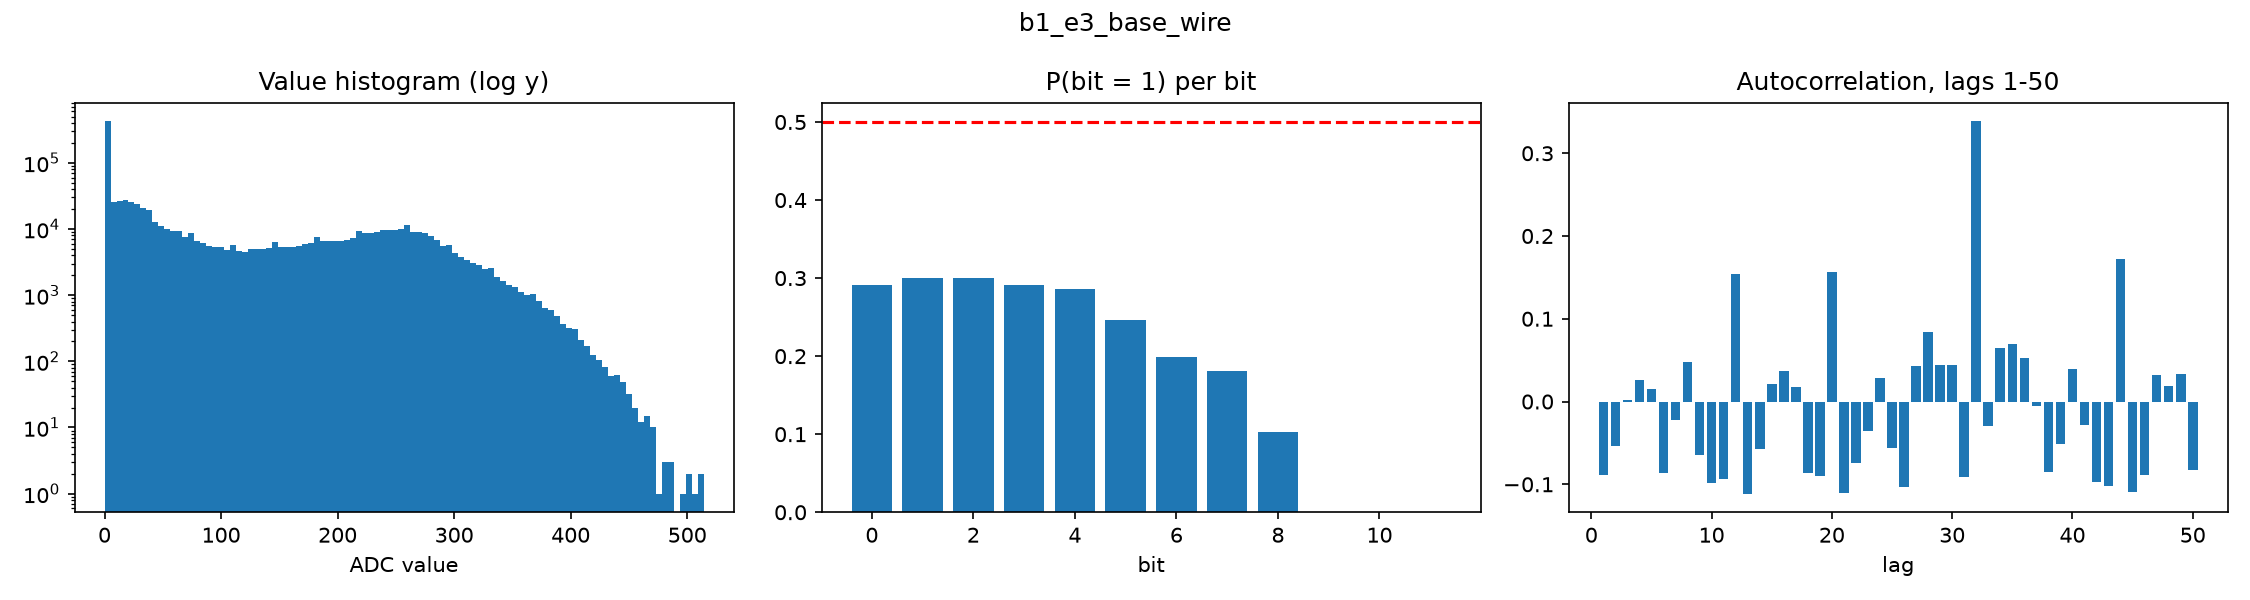
\includegraphics[width=\textwidth]{figures/b1_e3_base_wire.png}
\caption{Board 1, floating pin with a 10~cm wire attached. The distribution extends to larger values than in Figure~\ref{fig:bp_float_b1}.}
\label{fig:bp_wire}
\end{figure}
 
\subsubsection{Experiment 6: Dependence of the Measurement on Host Activity}
 
\paragraph{Observation.} The autocorrelation of every floating-pin capture contains a dominant peak at lag 32 (about 0.55 for B1 run r4, 0.75 for B2, and 0.34 with the wire attached; Figures~\ref{fig:bp_float_b1}, \ref{fig:bp_float_b2} and \ref{fig:bp_wire}), whereas the internal temperature sensor and the grounded pin show no such peak.
 
\paragraph{Method.} A hypothesis I presented was that the periodicity came from the board's own serial transmission, which paces the sampling loop. To test it, a second firmware sampled 4,000 readings into RAM while the UART was idle, and transmitted them afterwards. Two streaming captures were taken before and after the burst capture, without moving the board.
  
\begin{table}[htbp]
\centering
\small
\caption{Streaming versus burst sampling of the floating pin of B1}
\label{tab:bp_e6}
\begin{tabularx}{\textwidth}{@{}Xccc@{}}
\toprule
\textbf{Capture} & \textbf{Autocorrelation at lag 32} & \textbf{Mean reading} & \textbf{Min-entropy} \\
\midrule
Streaming (before) & 0.927 & 43.7 & 1.898 \\
Burst, UART idle while sampling & $-0.000$ & 28.9 & 1.052 \\
Streaming (after) & 0.926 & 43.7 & 1.868 \\
\bottomrule
\end{tabularx}
\end{table}
 
The two streaming captures agree closely, so the setup was stable. The lag 32 peak vanishes in the burst capture, the mean falls by about 15 counts, and the min-entropy falls by about 0.8 bits. The burst capture also contained 1,000 outlier readings (above 2000) at exactly four fixed positions in every 4,000-sample burst, which was not further investigated.
 
\paragraph{Discussion.} The result suggests that the host's own activity does affects what the floating pin reads, and that the measured entropy of this source depends on how it is sampled. The explanation is a hypothesis and not a proven cause as such, since the burst method also changes the sampling rate and timing. If the board's own switching activity contributes to the signal, that part is deterministic and could be influenced, so it cannot be treated as unpredictable. For this reason no single min-entropy figure can be claimed for the floating pin.
 
\subsubsection{Experiment 7: SRAM Start-up State}
 
\paragraph{Method.} The state of SRAM after power-up is the one entropy source of the chip that needs no peripheral, and it has been reported to hold substantial entropy on related STM32 devices \citep{cryptoeprint:2013/304}. The firmware copied a 4~KB region of otherwise unused SRAM at the very start of start-up and sent it to the laptop. 20 captures were taken per board, each after a full power-off (both USB connections removed for more than 10 seconds). The 4~KB region was checked to confirm it held start-up data and not a cleared region. The stability of each bit across captures, the Hamming distance between captures, and a rough per bit min-entropy sum were computed.
 
\paragraph{Results.} Table~\ref{tab:bp_e7} gives the results.
 
\begin{table}[htbp]
\centering
\small
\caption{SRAM start-up state, 20 power cycles per board, 32,768 bits per capture}
\label{tab:bp_e7}
\begin{tabularx}{\textwidth}{@{}Xcc@{}}
\toprule
 & \textbf{B1} & \textbf{B2} \\
\midrule
Fraction of bits equal to 1 & 0.478 & 0.495 \\
Bits identical in all 20 captures & 82.1\% & 82.2\% \\
Mean Hamming distance between captures & 5.36\% & 5.39\% \\
Rough min-entropy per capture & 2,062 bits & 2,080 bits \\
\multicolumn{3}{@{}l}{Hamming distance between a B1 capture and a B2 capture: 49.92\%} \\
\bottomrule
\end{tabularx}
\end{table}
 
\paragraph{Observations.} Most of the SRAM (82\%) takes the same value at every power-up, so it acts as a board specific fingerprint and only a minority of cells vary between power cycles. The two boards' patterns are unrelated (distance close to 50\%). The varying cells carry roughly 2,000 bits of min-entropy per 4~KB by this rough measure. This estimate is preliminary with only 20 power cycles, a cell that happened to stay constant is credited with zero entropy and the estimate for the varying cells is itself uncertain, therefore more power cycles maybe needed for a definitive measurement.
 
\paragraph{Discussion.} SRAM start up is the strongest local source measured, and could in principle seed a key on its own after a clean power up. Its limitations are those of a one shot source: it is available only at power-on (a warm reset keeps the old contents), the stable portion is predictable to anyone who can read the memory of the same board, and it must be characterised per board. These measurements do not show how it behaves across temperature and supply voltage. A summary figure is shown in Figure~\ref{fig:bp_sram}.
 
\begin{figure}[htbp]
\centering
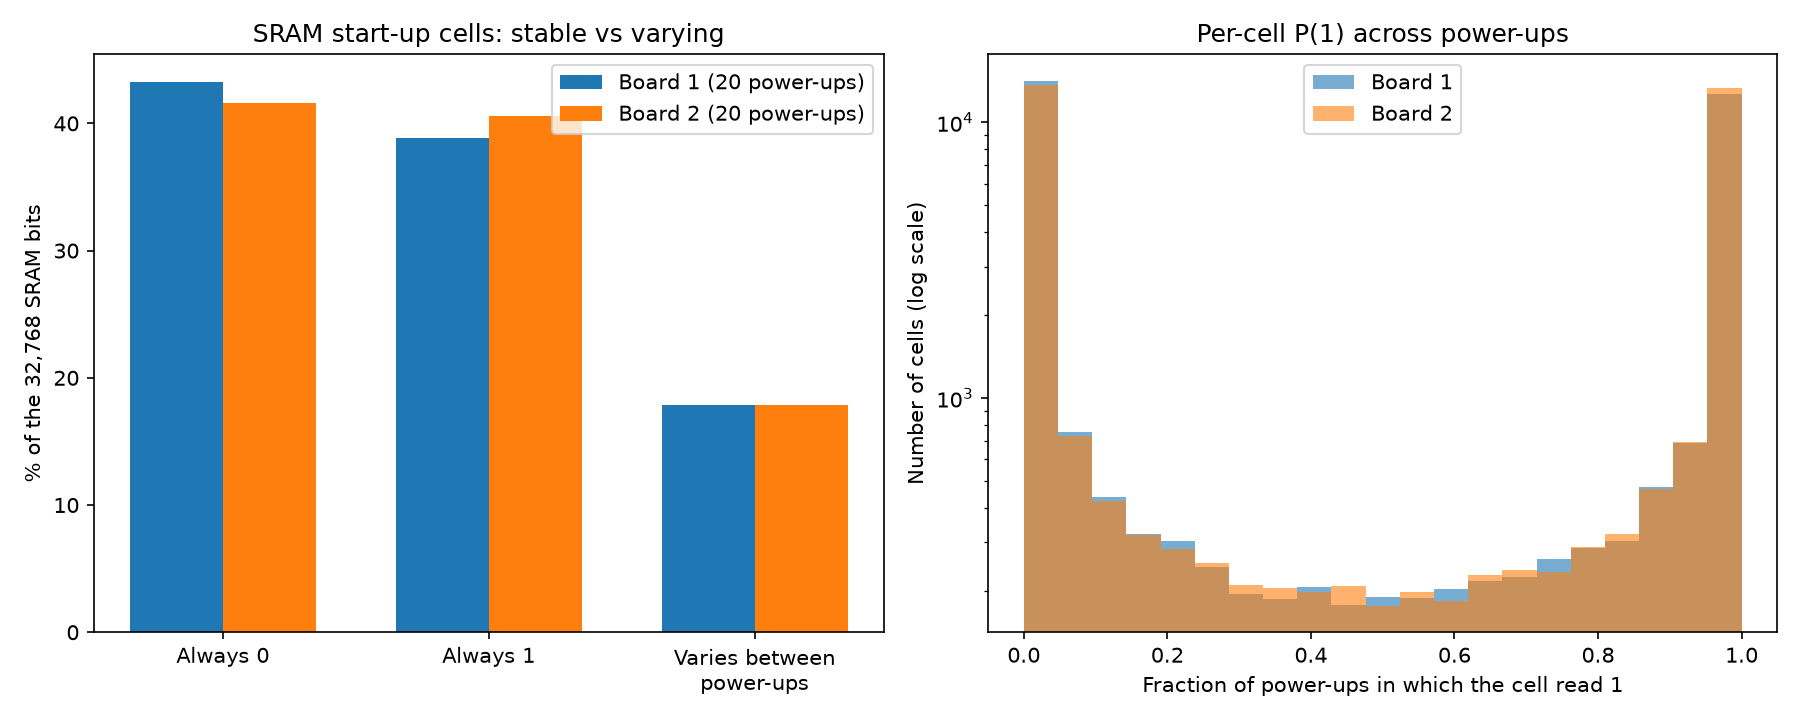
\includegraphics[width=\textwidth]{figures/sram_cells.png}
\caption{SRAM start-up cells over 20 power-ups: proportion of cells that are always 0, always 1, or vary (left), and the distribution of the per-cell probability of reading 1 (right, logarithmic scale). ``Always'' means constant in these 20 captures.}
\label{fig:bp_sram}
\end{figure}
 
\subsubsection{Summary of Findings}
 
Table~\ref{tab:bp_summary} consolidates the results and the confidence I place in each.
 
\begin{table}[htbp]
\centering
\small
\caption{Summary of findings from the single-device experiments}
\label{tab:bp_summary}
\begin{tabularx}{\textwidth}{@{}p{0.31\textwidth}Xp{0.22\textwidth}@{}}
\toprule
\textbf{Finding} & \textbf{Evidence} & \textbf{Limitations} \\
\midrule
Common seeding practices give identical, predictable output on every boot and across devices & Exp.~1: one distinct value in 100 boots for four seed types, on both boards & Software resets, two boards \\
A single analogue reading as seed reduces a 128-bit key to a handful of values & Exp.~3: 5 distinct keys in 500 boots; all recovered with a 4,095-entry table & One board, attacker knows firmware \\
Output statistics cannot reveal the above & Exp.~2: identical stream on both boards scored 6.97 bits per byte & Tool is meant for physical sources \\
Raw analogue sources give about 1 to 2.4 bits per 8-bit sample & Exp.~4: both boards, 3 runs per source & Varies with board and setup \\
The converter alone contributes almost nothing & Exp.~4: grounded pin below 0.01 bits & Origin of the floating-pin signal\\
Floating-pin quality depends on mounting and on how it is sampled & Exp.~5 and 6 & Single board, hypothesis for cause \\
SRAM start-up is the strongest local source but is one-shot and board-specific & Exp.~7: about 2,000 bits per 4~KB; 82\% of bits stable & 20 power cycles, preliminary estimate \\
\bottomrule
\end{tabularx}
\end{table}
 
\subsubsection{Implications for the Proposed Design}
\label{sec:bp_implications}
 
\begin{itemize}
    \item \textbf{No single local source can be trusted.} Every source is weak, variable, or available only once, which supports a design that combines several inputs and does not depend on one of them. This is consistent with the defence-in-depth argument made for boot entropy by \citet{blancoromero2026bootstrap}.
    \item \textbf{Local entropy must be credited conservatively.} Because the quality of a local source varies and cannot be verified from its output, the entropy credited to each input should come from evidence, and credit for several inputs should not be summed unless their independence is verified.
    \item \textbf{Weak local entropy is not zero.} The measurements show that devices usually has \emph{some} unpredictability locally. The mechanism being developed should therefore combine this with entropy from peers so that a seed remains unpredictable as long as at least one contribution is unknown to the attacker, rather than relying on peers to supply all of it.
    \item \textbf{Evaluation must examine raw inputs.} Since output tests cannot reveal predictability, the evaluation plan measures min-entropy on the raw local and peer contributions, together with adversarial scenarios, and not only statistical test results on the final output.
    \item \textbf{One-shot sources leave a gap.} Since SRAM is available only at power-on, devices that restart without power loss have no comparable source, which a peer exchange can fill.
\end{itemize}
 
\subsubsection{Limitations}
 
\begin{itemize}
    \item Only two boards were tested, and are probably from the same batch. Differences between them are observations and not statements about the entire chip family.
    \item Boot-time experiments used software resets and not power cycles. The NIST restart test, which assesses entropy immediately after reset, has not yet been carried out.
    \item Floating-pin results depend strongly on setup and on sampling method.
    \item The SRAM min-entropy figure is a rough estimate from 20 power cycles, and temperature and voltage were not varied.
    \item Estimates were made after reducing 12-bit readings to 8 bits, and the estimator is designed for independent physical noise sources and is applied here to sources with strong dependence.
\end{itemize}
 
\subsubsection{Conclusion and Next Steps}
 
The experiments on two real boards show that a constrained device without a hardware random number generator is a weak source of randomness when used in the ways that are common in practice. Typical seeding produces identical output across devices, a single analogue reading collapses a nominal 128-bit key to a few values that an attacker recovers instantly, output statistics cannot reveal the weakness, the raw analogue sources provide roughly one to two bits of min-entropy per sample. These results justify the research problem and give the baseline against which the proposed collaborative mechanism will be compared. They also show that a single local entropy source cannot be trusted, and that the proposed combination of local and peer entropy should be designed on the assumption that every input is weak and unverifiable.
 
The next stage would address the first research question: a lightweight peer-to-peer exchange over a low cost 2.4~GHz radio module, whose hardware setup on the boards has begun, followed by a simulation of the protocol for different node counts and loss rates, and measurement of delivery rate, latency and overhead on the boards. The adversarial trust model and the full evaluation against these baselines follow as described in the Evaluation Plan.

\section{Evaluation Plan}
\subsection{Purpose and Scope of the Evaluation}
 
My evaluation has to show with evidence, that the proposed mechanism for combining locally harvested entropy with peer-contributed entropy (1) works on resource constrained devices without a central server, (2) improves the randomness available to a device compared with what it can obtain alone, (3) remains safe when some participants are biased or malicious and (iv) compares favourable manner with established alternatives. The four claims correspond directly to the four research questions, and each is evaluated separately so that a negative result on one does not hide a positive result on another.
 
The evaluation follows the experimental evaluation stage of the design science approach adopted for this research \citep{hevner2004design,peffers2007dsrm}. The artifact (protocol, mixing mechanism and the trust model) is built, demonstrated and then measured against set objectives and baselines. The measurements already made on the single-device platform (Section~\ref{sec:bluepill}) form the baseline and also will supply data to the simulations.
 
\subsection{Evaluation Questions, Metrics and Evidence}
  
\begin{table}[htbp]
\centering
\small
\caption{Evaluation matrix}
\label{tab:ev_matrix}
\begin{tabularx}{\textwidth}{@{}p{0.07\textwidth}p{0.3\textwidth}Xp{0.17\textwidth}@{}}
\toprule
\textbf{RQ} & \textbf{Metrics} & \textbf{How measured} & \textbf{Environment} \\
\midrule
RQ1 &
Delivery success rate, latency from request to seed, messages and bytes per round per node, flash and RAM usage, hashing and mixing time, energy per round (if instrument is available) &
current measured with an INA219 module, Logged counters and timestamps
on each node
 & 
Testbed and simulation \\
\addlinespace
RQ2 &
Credited min-entropy of each input and of the final seed, time (rounds) to reach the target credited entropy, seed uniqueness across boots and nodes &
SP~800-90B estimates on the raw inputs; credit accounting as defined by the mixing rule; number of distinct seeds in repeated boots (as in Experiment~1 and 3) &
Testbed and simulation \\
\addlinespace
RQ3  &
Detection rate, false positive rate, rounds until detection, honest-node seed strength when $f$ peers are malicious, effective attacker search space &
Injected adversaries with known ground truth, confusion matrix for scenario, key recovery attacks &
Simulation first, then testbed \\
\addlinespace
RQ4  &
Above metrics for the proposed mechanism and for baselines, across node counts and adversary levels &
Same scenarios, same random seeds and same measurement tooling for every method &
Testbed and simulation \\
\bottomrule
\end{tabularx}
\end{table}
 
\paragraph{Why the output of the mixer is not used as evidence.} The experiments in Section 5 showed that statistical analysis of a generator's output cannot reveal a lack of unpredictability, a fully predictable stream scored 6.97 bits per byte. Hashing the mixed inputs will make almost any combination look random. The evaluation therefore measures the \emph{inputs}, credits entropy only from evidence about them, and checks the guarantee directly against adversaries. Statistical tests on the final output (for example ENT and the SP~800-90B tool) are run only as sanity checks and are reported as such.
 
\subsection{Evaluation Environments}
 
Two environments are used with the testbed showing that the mechanism runs on real constrained hardware, while only simulation can reach larger networks, many repetitions and adverserial control.
 
\paragraph{Hardware testbed.} Four to five nodes, each with an nRF24L01+ 2.4~GHz radio module, running the protocol on a RTOS. The nodes are within radio range of each other (single hop). A laptop records logs from the nodes over UART.
 
\paragraph{Simulation.} A Simulator models $N$ nodes exchanging messages over a lossy, delayed link, using the same message formats, packet size limit (32 bytes) and timeouts as the testbed. Link loss and latency are calibrated from the radio measurements on the testbed. Each simulated node draws its local entropy from \emph{empirical data}: the raw captures from Experiments~4 and 7 (floating pin, temperature sensor, SRAM start-up)
 
\subsection{Adversary Model and Scenarios}
 
The attacker is assumed to be knowing the firmware and all protocol parameters, to be able to observe the radio channel (unless the link is protected), and to control up to $f$ of the $N$ participating nodes. The attacker cannot read the internal memory of honest nodes. The guarantee evaluated is that a node's seed remains unpredictable as long as at least one input to it is unknown to the attacker.
 
\begin{table}[htbp]
\centering
\small
\caption{Planned Evaluation scenarios}
\label{tab:ev_scenarios}
\begin{tabularx}{\textwidth}{@{}p{0.06\textwidth}p{0.27\textwidth}X@{}}
\toprule
\textbf{ID} & \textbf{Scenario} & \textbf{Description and levels} \\
\midrule
S0 & Benign network & All nodes honest; $N$ varied; packet loss 0, 10 and 30\%. \\
S1 & Passive eavesdropper & Attacker records every message. Evaluated with and without link protection, to show how much of the benefit depends on the link being private. \\
S2 & Stuck contributors & $f$ nodes send constant or repeating values. \\
S3 & Biased contributors & $f$ nodes send bit-biased values, with the bias level varied. \\
S4 & Replay & Attacker re-sends messages from earlier rounds. \\
S5 & Adaptive (last-mover) contributor & A malicious node sees other contributions before choosing its own, trying to steer the result. \\
S6 & Colluding minority & $f$ malicious nodes coordinate their contributions. \\
S7 & Dominant strong node & One high-resource node supplies most of the entropy, honest in one run and compromised in another. Shows how much the network depends on it. \\
S8 & Loss and delay & Dropped, delayed or withheld messages, including a node that withholds its reveal. \\
\bottomrule
\end{tabularx}
\end{table} 
 
\begin{table}[htbp]
\centering
\small
\caption{Baselines}
\label{tab:ev_baselines}
\begin{tabularx}{\textwidth}{@{}p{0.06\textwidth}p{0.26\textwidth}X@{}}
\toprule
\textbf{ID} & \textbf{Method} & \textbf{Purpose} \\
\midrule
B0 & Local only (each measured source, and SRAM start-up) & Shows what a device achieves alone. Already measured in Section 5 \\
B1 & Common seeding practices (fixed seed, time, one analogue reading) & Reproduces the predictability measured in Experiments~1 and 3. \\
B2 & Trusted gateway (entropy-as-a-service style) & One strong node supplies the entropy to the others \citep{NIST_EaaS}. Shows the benefit and the single-point-of-failure risk of a central source. \\
B3 & Naive peer mixing (XOR or plain hash of all received values, with no trust model or commitment) & Showing what the trust and commitment mechanisms add. \\
A1--A3 & Proposed mechanism with one component removed at a time (commitment step; contribution cap and minimum number of distinct peers; local entropy always mixed in) & Shows which design choices are needed, and justifies each of them. \\
\bottomrule
\end{tabularx}
\end{table}
 
\subsection{Experimental Design}
 
\paragraph{Factors and levels.} Table~\ref{tab:ev_factors} lists the factors varied. Not every combination is run.
 
\begin{table}[htbp]
\centering
\small
\caption{Experimental factors}
\label{tab:ev_factors}
\begin{tabularx}{\textwidth}{@{}p{0.3\textwidth}p{0.18\textwidth}X@{}}
\toprule
\textbf{Factor} & \textbf{Environment} & \textbf{Levels} \\
\midrule
Number of nodes $N$ & Simulation & 3, 5, 10, 20, 50 \\
Number of nodes $N$ & Testbed & 2, 3, 4, 5 \\
Malicious fraction $f/N$ & Both & 0, about 20, 40 and 60\% (rounded to whole nodes) \\
Packet loss & Both & 0, 10, 30\% \\
Local entropy source & Both & Floating pin, temperature sensor, SRAM start-up (measured data) \\
Method & Both & Proposed mechanism, B0 to B4 \\
\bottomrule
\end{tabularx}
\end{table}
 
\paragraph{Repetitions.} Each simulated configuration is repeated at least 30 times with different random seeds, and every seed is logged so that runs can be reproduced. On the testbed, each configuration is run for at least 100 protocol rounds. Mean and spread are reported.
 
\paragraph{Data collection and integrity.} The data pipeline established for the baseline experiments is reused. Every capture is logged with date, board, firmware version and physical conditions; saved files are hashed; framing, range and duplicate checks are applied; and any capture that fails a check is discarded and recorded as excluded.
 
\subsection{Procedure for Each Research Question}
 
\paragraph{RQ1: lightweight exchange.}
\begin{enumerate}
    \item Verify the radio link between two nodes and measure raw packet loss and round trip time at several distances and channels.
    \item Run the request and contribution exchange on 2 to 5 nodes and record, for each round, whether the requester received the required number of valid contributions, and the time taken.
    \item Record flash and RAM use from the build output, CPU time of the mixing step
    \item Calibrate the simulator with the measured loss and latency, and compare simulated and measured delivery and latency on the same configurations. Differences are reported and explained.
    \item Use the simulator to extend the results to larger $N$.
\end{enumerate}
 
\paragraph{RQ2: combining local and peer entropy.}
\begin{enumerate}
    \item For each local source, take the min-entropy estimate from the baseline measurements as the credited entropy of that source.
    \item Under the mixing rule, compute the credited entropy of the final seed with 0, 1, 2 and 3 or more peers, and the number of rounds needed to reach the target (for example 128 and 256 bits).
    \item Repeat the key-recovery attack of Experiment~3 on seeds produced by the mechanism, and report the effective search space and the number of distinct seeds over many boots, compared with B1.
    \item Run ENT and SP~800-90B tests on the final output as a sanity check.
\end{enumerate}
 
\paragraph{RQ3: malicious or biased contributors.}
\begin{enumerate}
    \item Inject adversaries for scenarios in the simulator with known ground truth.
    \item Record detection rate, false positive rate and rounds to detection for the trust model.
    \item For each scenario, compute the credited entropy of an honest node's seed using only the honest contributions, to show that the guarantee holds when a minority of nodes cheat.
    \item Reproduce selected scenarios on the testbed
\end{enumerate}
 
\paragraph{RQ4: comparison with baselines.} Run the proposed mechanism and baselines B0 to B3 over the same scenarios, node counts and random seeds, and compare credited entropy, time to seed, detection and overhead.


 
\subsection{Limitations}
 
\begin{itemize}
    \item \textbf{Setup sensitivity.} The baseline measurements showed that the floating-pin entropy changes with mounting and contact. Mitigation: compare methods only within one session, re-measure baselines in each session, and log conditions. Where possible, prefer sources less sensitive to setup (for example the SRAM start-up state).
    \item \textbf{Simulation versus reality.} The simulator uses measured loss, latency and entropy data but is still a model. Simulated and measured results are compared on the configurations where both exist.
    \item \textbf{Measuring entropy.} SP~800-90B was designed for physical noise sources, and the sources here are strongly dependent and reduced to 8 bits for the tool. The lowest estimator value is reported, and entropy credit is deliberately conservative.
    \item \textbf{Attacker model.} Scenarios S1 to S8 are possible attack scenarios. some attack scenarios may enter or move out of scope with the time feasible.
    \item \textbf{Baseline fidelity.} Baselines B2 to B4 are reproduced from their descriptions and are simplified. They are labelled as approximations.
    \item \textbf{Statistical power.} With minimal physical nodes, large-network claims rest on simulation only.
\end{itemize}
 
\subsection{Tools and Reproducibility}
 
All code, scenario configurations and other artifacts are kept in a version-controlled repository.
 
\subsection{Evaluation Timeline}
 
The evaluation proceeds in the following order, consistent with my adaptive research timeline
 
\begin{enumerate}
    \item \textbf{Completed:} single-device baseline (Section~\ref{sec:bluepill}).
    \item Radio link and the first two-node exchange (RQ1).
    \item Simulator implementation, calibration with testbed measurements, and RQ1 results at larger $N$.
    \item Mixing mechanisms (RQ2).
    \item Adversary scenarios and trust model evaluation, in simulation and then on the testbed (RQ3).
    \item Full comparison with baselines. (RQ4)
\end{enumerate}
 
If evaluation step shows anomalies or the criteria are not met, the process will loops back to the design as per the timeline.





\begin{landscape}

 
\vspace{0.3em}
\renewcommand{\arraystretch}{1.15}
\setlength{\tabcolsep}{3pt}
\captionof{table}{Adaptive Research Timeline}
\scriptsize
\begin{tabularx}{\linewidth}{|p{1.5cm}|X|X|X|}
\hline
\rowcolor{headerblue}
\textbf{Tracks} & \textbf{(Months 1--3)} & \textbf{(Months 4--8)} & \textbf{(Months 9--10)} \\
\hline
 
\textbf{Core} &
\makecell[l]{Problem identification \\ Building the foundation \\ Critical analysis of work} &
 & \\
\hline
 
\textbf{Research} &
\makecell[l]{Main Research Drive \\ Solution Gaps \& Limitations \\ Refining Research Questions} &
\makecell[l]{$\rightarrow\!\rightarrow\!\rightarrow$ Continuous Gap Refinement \\ $\rightarrow\!\rightarrow\!\rightarrow$ Adaptive RQ Optimization} &
\\
\hline
 
\textbf{Phases} &
 &
\makecell[l]{Execution of methodology \\ Tooling, Datasets and modifications} &
\makecell[l]{\textbf{Evaluation Procedure} \\ \& Metric Justification} \\
\hline
 
\rowcolor{lightblue}
\textbf{Phase-Gate} &
{[Taxonomy of Gap \& Finalized RQs]} &
{[Modified Framework \& Core system]} &
{[Evaluation Results]} \\
\hline
 
\textbf{Feedback} &
 &
\makecell[l]{$\circ$ \textbf{IF} data limitations emerge,\\ \textbf{LOOP BACK} to\\ re-scope approach.} &
\makecell[l]{$\circ$ \textbf{IF} evaluation drops anomalies,\\ \textbf{LOOP BACK} to\\ re-calibrate tools.} \\
\hline
 
\multicolumn{4}{|c|}{\cellcolor{headerblue}\textbf{Parallel Supporting Tracks (Continuous)}} \\
\hline
 
\rowcolor{headerblue}
\textbf{Tracks} & \textbf{(Months 1--3)} & \textbf{(Months 4--8)} & \textbf{(Months 9--10)} \\
\hline
 
\textbf{Literature Review} &
\makecell[l]{\textbf{[Heavy Focus]}\\Build taxonomy of work\\models and map the core gaps.} &
\makecell[l]{$\rightarrow\!\rightarrow\!\rightarrow$ \textbf{[Monitoring \& Comparison]}\\Scan for newly published studies;\\update gap analysis dynamically.} &
\makecell[l]{$\rightarrow\!\rightarrow\!\rightarrow$ \textbf{[Contextual Integration]}\\Map final evaluation data\\back against literature base.} \\
\hline
 
\textbf{Documen-tation} &
\makecell[l]{\textbf{[Drafting]}\\Write Intro, Problem Background,\\and initial Literature Review.} &
\makecell[l]{$\rightarrow\!\rightarrow\!\rightarrow$ \textbf{[Evolving]}\\Update Methodology logs as\\data deviations or new papers\\change path.} &
\makecell[l]{$\rightarrow\!\rightarrow\!\rightarrow$ \textbf{[Compiling \& Polishing]}\\Write Evaluation, Discussion,\\and finalize thesis formatting.} \\
\hline
 
\end{tabularx}
 
\end{landscape}
 



% ----------------------------------------
% References (Harvard)
% ----------------------------------------
\clearpage

\printbibliography

% ----------------------------------------
% Index (required)
% ----------------------------------------
\clearpage
% \section*{Index}
% \addcontentsline{toc}{section}{Index}

\end{document}
